% I seguenti commenti speciali impostano:
% 1. 
% 2. PDFLaTeX come motore di composizione;
% 3. tesi.tex come documento principale;
% 4. il controllo ortografico italiano per l'editor.

% !TEX encoding = UTF-8
% !TEX TS-program = pdflatex
% !TEX root = tesi.tex
% !TEX spellcheck = it-IT
%!TEX program = xelatex
\documentclass[11pt,                    % corpo del font principale
    a4paper,                 % carta A4
    twoside,                 % impagina per fronte-retro
    openright,               % inizio capitoli a destra
    english,
    ctexart,
]{book}

%**************************************************************
% Importazione package
%************************************************************** 
%\usepackage{amsmath,amssymb,amsthm}    % matematica
\usepackage[UTF8]{ctex}
\usepackage[T1]{fontenc}                % codifica dei font:
% NOTA BENE! richiede una distribuzione *completa* di LaTeX

\usepackage[utf8]{inputenc}             % codifica di input; anche [latin1] va bene
% NOTA BENE! va accordata con le preferenze dell'editor

\usepackage[english]{babel}    % per scrivere in italiano e in inglese;
% l'ultima lingua (l'italiano) risulta predefinita

\usepackage{bookmark}                   % segnalibri

\usepackage{caption}                    % didascalie

\usepackage{chngpage,calc}              % centra il frontespizio

\usepackage{csquotes}                   % gestisce automaticamente i caratteri (")

\usepackage{emptypage}                  % pagine vuote senza testatina e piede di pagina

\usepackage{epigraph}            % per epigrafi

\usepackage{eurosym}                    % simbolo dell'euro

%\usepackage{indentfirst}               % rientra il primo paragrafo di ogni sezione

\usepackage{graphicx}                   % immagini

\usepackage{hyperref}                   % collegamenti ipertestuali

\usepackage[binding=5mm]{layaureo}      % margini ottimizzati per l'A4; rilegatura di 5 mm


\usepackage{microtype}                  % microtipografia

\usepackage{mparhack,fixltx2e,relsize}  % finezze tipografiche

\usepackage{nameref}                    % visualizza nome dei riferimenti                                      

\usepackage[font=small]{quoting}        % citazioni

%\usepackage{subfig}                     % sottofigure, sottotabelle

\usepackage[english]{varioref}          % riferimenti completi della pagina

\usepackage[dvipsnames]{xcolor}         % colori
\usepackage{formattazione}

\usepackage{booktabs}                   % tabelle                                       
\usepackage{tabularx}                   % tabelle di larghezza prefissata                                    
\usepackage{longtable}                  % tabelle su più pagine                                        
\usepackage{ltxtable}                   % tabelle su più pagine e adattabili in larghezza

\usepackage{multicol}                   % colonne multiple
\usepackage{tabularx}

\usepackage{amsmath,bm}
\usepackage{version}
\usepackage{lscape}
\usepackage{listings}                   % for code listings

\usepackage[toc, acronym]{glossaries}   % glossario
% per includerlo nel documento bisogna:
% 1. compilare una prima volta tesi.tex;
% 2. eseguire: makeindex -s tesi.ist -t tesi.glg -o tesi.gls tesi.glo
% 3. eseguire: makeindex -s tesi.ist -t tesi.alg -o tesi.acr tesi.acn
% 4. compilare due volte tesi.tex.
\usepackage[backend=biber,style=numeric-comp,hyperref,backref]{biblatex}
% eccellente pacchetto per la bibliografia;
% produce uno stile di citazione autore-anno;
% lo stile "numeric-comp" produce riferimenti numerici
% per includerlo nel documento bisogna:
% 1. compilare una prima volta tesi.tex;
% 2. eseguire: biber tesi
% 3. compilare ancora tesi.tex.

%**************************************************************
% file contenente le impostazioni della tesi
%**************************************************************

%**************************************************************
% Frontespizio
%**************************************************************

% Autore
\newcommand{\myName}{Giuseppe Boezio}
\newcommand{\myTitle}{Labeled Prolog: a computational model in 2p-KT}

% Tipo di tesi                   
\newcommand{\myDegree}{Master degree thesis}

% Università             
\newcommand{\myUni}{Alma Mater Studiorum - University of Bologna}

% Facoltà       
\newcommand{\myFaculty}{Artificial Intelligence}

% Dipartimento
\newcommand{\myDepartment}{Computer Science and Engineering - DISI}

% Titolo del relatore
\newcommand{\profTitle}{Prof.}

% Relatore
\newcommand{\myProf}{Roberta Calegari}

% Luogo
\newcommand{\myLocation}{Bologna}

% Anno accademico
\newcommand{\myAA}{2021-2022}

% Data discussione
\newcommand{\myTime}{03 February 2023}


\addto\captionsenglish{\renewcommand{\lstlistingname}{Code}}

%**************************************************************
% Impostazioni di impaginazione
% see: http://wwwcdf.pd.infn.it/AppuntiLinux/a2547.htm
%**************************************************************

\setlength{\parindent}{14pt}   % larghezza rientro della prima riga
\setlength{\parskip}{0pt}   % distanza tra i paragrafi


%**************************************************************
% Impostazioni di biblatex
%**************************************************************
\bibliography{bibliografia} % database di biblatex 

\defbibheading{bibliography} {
    \cleardoublepage
    \phantomsection 
    %\addcontentsline{toc}{chapter}{\bibname}
    \chapter*{\bibname\markboth{\bibname}{\bibname}}
}

\setlength\bibitemsep{1.5\itemsep} % spazio tra entry

\DeclareBibliographyCategory{opere}
\DeclareBibliographyCategory{web}

\addtocategory{opere}{womak:lean-thinking}
\addtocategory{web}{site:agile-manifesto}

\defbibheading{opere}{\section*{Bibliography}}
\defbibheading{web}{\section*{Websites}}


%**************************************************************
% Impostazioni di caption
%**************************************************************
\captionsetup{
    tableposition=top,
    figureposition=bottom,
    font=small,
    format=hang,
    labelfont=bf
}

%**************************************************************
% Impostazioni di glossaries
%**************************************************************
\input{Glossario} % database di termini
\makeglossaries


%**************************************************************
% Impostazioni di graphicx
%**************************************************************
\graphicspath{{images/}} % cartella dove sono riposte le immagini


%**************************************************************
% Impostazioni di hyperref
%**************************************************************
\hypersetup{
    %hyperfootnotes=false,
    %pdfpagelabels,
    %draft,	% = elimina tutti i link (utile per stampe in bianco e nero)
    colorlinks=true,
    linktocpage=true,
    pdfstartpage=1,
    pdfstartview=FitV,
    % decommenta la riga seguente per avere link in nero (per esempio per la stampa in bianco e nero)
    %colorlinks=false, linktocpage=false, pdfborder={0 0 0}, pdfstartpage=1, pdfstartview=FitV,
    breaklinks=true,
    pdfpagemode=UseNone,
    pageanchor=true,
    pdfpagemode=UseOutlines,
    plainpages=false,
    bookmarksnumbered,
    bookmarksopen=true,
    bookmarksopenlevel=1,
    hypertexnames=true,
    pdfhighlight=/O,
    %nesting=true,
    %frenchlinks,
    urlcolor=webbrown,
    linkcolor=RoyalBlue,
    citecolor=webgreen,
    %pagecolor=RoyalBlue,
    %urlcolor=Black, linkcolor=Black, citecolor=Black, %pagecolor=Black,
    pdftitle={\myTitle},
    pdfauthor={\textcopyright\ \myName, \myUni, \myFaculty},
    pdfsubject={},
    pdfkeywords={},
    pdfcreator={pdfLaTeX},
    pdfproducer={LaTeX}
}

%**************************************************************
% Impostazioni di listings
%**************************************************************
\lstset{
    language=[LaTeX]Tex,%C++,
    keywordstyle=\color{RoyalBlue}, %\bfseries,
    basicstyle=\small\ttfamily,
    %identifierstyle=\color{NavyBlue},
    commentstyle=\color{Green}\ttfamily,
    stringstyle=\rmfamily,
    numbers=none, %left,%
    numberstyle=\scriptsize, %\tiny
    stepnumber=5,
    numbersep=8pt,
    showstringspaces=false,
    breaklines=true,
    frameround=ftff,
    frame=single
} 


%**************************************************************
% Impostazioni di xcolor
%**************************************************************
\definecolor{webgreen}{rgb}{0,.5,0}
\definecolor{webbrown}{rgb}{.6,0,0}
\usepackage{chngcntr}
\counterwithout{footnote}{chapter}

%**************************************************************
% Altro
%**************************************************************

\newcommand{\omissis}{[\dots\negthinspace]} % produce [...]

% eccezioni all'algoritmo di sillabazione
\hyphenation
{
    ma-cro-istru-zio-ne
    gi-ral-din
}

\newcommand{\sectionname}{Section}
\addto\captions{\renewcommand{\figurename}{Figure}
                       \renewcommand{\tablename}{Table}}

\newcommand{\glsfirstoccur}{\ap{{[g]}}}

\newcommand{\intro}[1]{\emph{\textsf{#1}}}

%**************************************************************
% Environment per ``namespace description''
%**************************************************************

\newenvironment{namespacedesc}{
    \vspace{10pt}
    \par \noindent                              % start new paragraph
    \begin{description} 
}{
    \end{description}
    \medskip
}

\newcommand{\classdesc}[2]{\item[\textbf{#1:}] #2}
\renewcommand{\labelitemi}{$\bullet$}
\renewcommand{\labelitemii}{$\circ$}
\renewcommand{\labelitemiii}{-}
\renewcommand{\labelitemiv}{$\cdot$}
                     % file con le impostazioni personali
\raggedbottom
\begin{document}
    %**************************************************************
    % Materiale iniziale
    %**************************************************************
    \frontmatter
    % !TEX encoding = UTF-8
% !TEX TS-program = pdflatex
% !TEX root = ../tesi.tex

%**************************************************************
% Frontespizio 
%**************************************************************
\begin{titlepage}

\begin{center}

\begin{LARGE}
\textbf{\myUni}\\
\end{LARGE}

\vspace{10pt}

\begin{Large}
\textsc{\myDepartment}\\
\end{Large}

\vspace{10pt}

\begin{large}
\textsc{\myFaculty}\\
\end{large}

\vspace{220pt}
%\begin{figure}[htbp]
%\begin{center}
%%\includegraphics[height=6cm]{logo}
%\end{center}
%\end{figure}
%\vspace{30pt}

\begin{LARGE}
\begin{center}
\textbf{\myTitle}\\
\end{center}
\end{LARGE}

\vspace{10pt} 

\begin{large}
\textsl{\myDegree}\\
\end{large}

\vspace{20pt}

\begin{large}
\begin{flushleft}
\textit{Supervisor}\\
\vspace{5pt} 
\profTitle \myProf\\
\textit{Co-supervisor}\\
\vspace{5pt}
Prof. Giovanni Ciatto
\end{flushleft}

\vspace{0pt} 

\begin{flushright}
\textit{Candidate}\\
\vspace{5pt} 
\myName
\end{flushright}
\end{large}

\vspace{20pt}

\line(1, 0){338} \\
\begin{normalsize}
\textsc{Academic Year \myAA - Third session}
\end{normalsize}

\end{center}
\end{titlepage}
    % !TEX encoding = UTF-8
% !TEX TS-program = pdflatex
% !TEX root = ../tesi.tex

%**************************************************************
% Colophon
%**************************************************************
\clearpage
\phantomsection
\thispagestyle{empty}

\hfill

\vfill

\noindent\myName: \textit{\myTitle,}
\myDegree,
\textcopyright\ \myTime.

\cleardoublepage
    % !TEX encoding = UTF-8
% !TEX TS-program = pdflatex
% !TEX root = ../tesi.tex

%**************************************************************
% Sommario
%**************************************************************
\cleardoublepage
\phantomsection
\pdfbookmark{Abstract}{Abstract}
\begingroup
\let\clearpage\relax
\let\cleardoublepage\relax
\let\cleardoublepage\relax

\chapter*{Abstract}

%\vfill
%
%\selectlanguage{english}
%\pdfbookmark{Abstract}{Abstract}
%\chapter*{Abstract}
%
%\selectlanguage{italian}
2P-Kt is an interpreter for Prolog language which is written in a way such that it can be easily extended and customized to deal with
specific needs. In the current scenario Constraint Logic Programming (CLP) has been supported by this system using an interface which is
as close as possible to the predicates' signatures used by famous and most used CLP(X) family of libraries supported by SWI Prolog interpreter.
A real case study concerning school timetabling is described to show a practical usage of CLP(FD) library implemented with the aforementioned 2P-Kt interpreter.
This case study shows how libraries have been modularized in such a way that they can be used as dependencies in every project developed for the Java
Virtual Machine (JVM).\newline
Constraint Logic Programming represents only a particular scenario for logic programming: for this reason a framework which extends the
mechanism of Labelled Variables has been implemented to show how it is possible to frame all variations and extensions of logic programming under a
single language reducing the huge amount of existing languages and libriaries and focusing on more on how to manage different domain needs using labels
which can be associated to every kind of term.
\endgroup

\vfill


    % !TEX encoding = UTF-8
% !TEX TS-program = pdflatex
% !TEX root = ../tesi.tex

%**************************************************************
% Indici
%**************************************************************
\cleardoublepage
\pdfbookmark{\contentsname}{tableofcontents}
\setcounter{tocdepth}{2}
\tableofcontents
%\markboth{\contentsname}{\contentsname} 
\clearpage

\begingroup 
    \let\clearpage\relax
    \let\cleardoublepage\relax
    \let\cleardoublepage\relax
    %*******************************************************
    % Elenco delle figure
    %*******************************************************    
    \phantomsection
    \pdfbookmark{\listfigurename}{lof}
    \listoffigures

    \vspace{8cm}

    %*******************************************************
    % Elenco delle tabelle
    %*******************************************************
    \phantomsection
    \pdfbookmark{\listtablename}{lot}
    \listoftables
    \vspace*{8ex}
\endgroup

\cleardoublepage

    \cleardoublepage

    %**************************************************************
    % Materiale principale
    %**************************************************************
    \mainmatter
    % !TEX encoding = UTF-8
% !TEX TS-program = pdflatex
% !TEX root = ../tesi.tex

%**************************************************************
\chapter{Introduction}\label{ch:introduction}
%**************************************************************

\intro{In this section we will present the summarized content of the whole thesis.}
%\noindent Esempio di utilizzo di un termine nel glossario \\
%\gls{api}. \\
%
%\noindent Esempio di citazione in linea \\
%\cite{site:agile-manifesto}. \\
%
%\noindent Esempio di citazione nel pie' di pagina \\
%citazione\footcite{womak:lean-thinking} \\

%**************************************************************

\section{Background}\label{sec:background}
Computer vision (CV) is a field of artificial intelligence that deals with the study of how computers can be made to gain high-level understanding from digital images or videos.
If AI allows the computer to think like a human as well as computer vision allows the computer to see like a human.

CV works like the human visual system, with the big difference in the fact that human uses year and year of experience to help the mind to understand what it is seeing.
As the biological neurons processes the information in the brain, the artificial neurons processes the information in the artificial neural network following the Hebbian plasticity (\cite{site:hebbian-plasticity}) rule: the connection between two neurons is strengthened if they are active at the same time.

In recent years, deep learning has revolutionized the CV field, achieving excellent results in many tasks, like: image classification, object detection, semantic segmentation, image captioning, image generation, etc.

The image classification task consists of assigning a label to an image with only one object (\hyperref[fig:figure-tulips]{Figure 1.1}).
\begin{figure}[H]
    \centering
    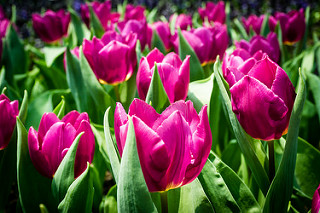
\includegraphics[width=0.8\textwidth]{images/1_1_tulips}
    \caption[Example of image classification]{Image classification: this image is classified as a tulip}
    \label{fig:figure-tulips}
\end{figure}
The object detection tasks consists of assigning a label and a bounding box to each object in the image.
The bounding box is a rectangle that encloses the object(\hyperref[fig:figure-object-detection]{Figure 1.2}).
\begin{figure}[H]
    \centering
    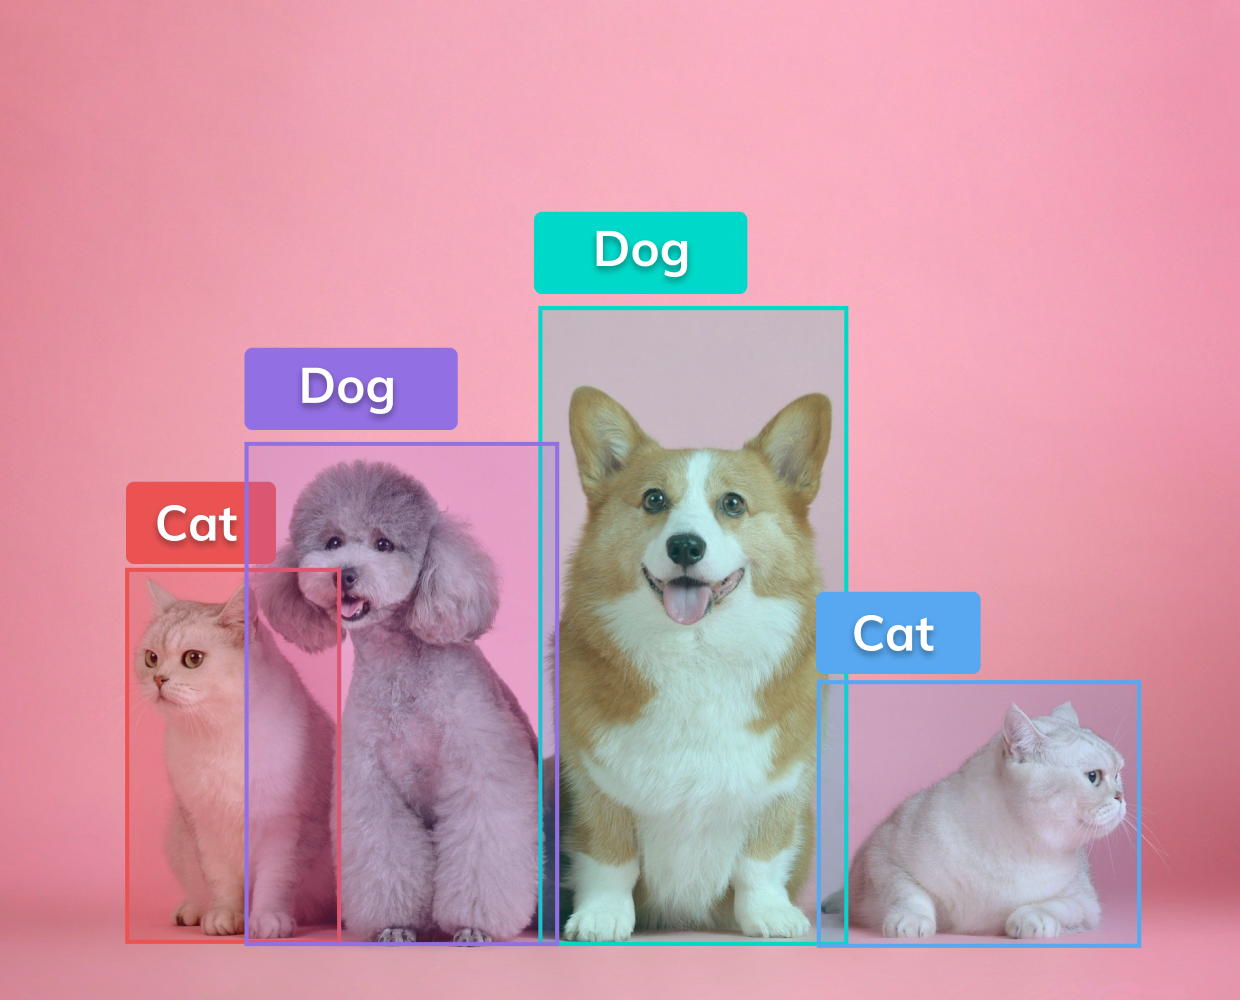
\includegraphics[width=0.8\textwidth]{images/1_1_object_detection}
    \caption[Example of object detection]{Object detection: this image contains two classes of objects, cat and dog.}
    \label{fig:figure-object-detection}
\end{figure}
The semantic segmentation task consists of assigning a label to each pixel of the image(\hyperref[fig:figure-semantic-segmentation]{Figure 1.3}).

\begin{figure}[H]
    \centering
    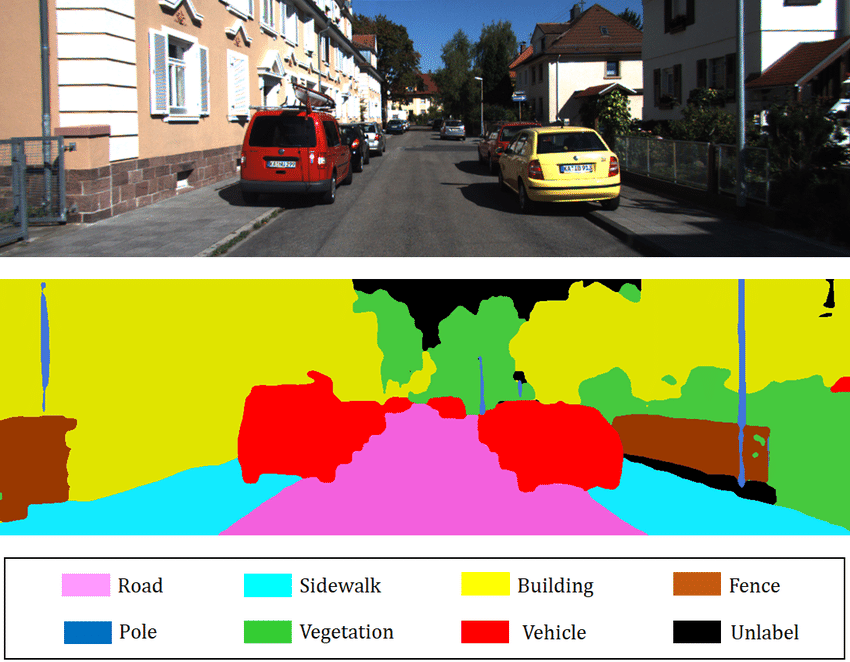
\includegraphics[width=0.8\textwidth]{images/1_1_semantic_segmentation}
    \caption[Example of semantic segmentation]{Semantic segmentation: each pixel is assigned a label.}
    \label{fig:figure-semantic-segmentation}
\end{figure}

Then, the modern CV systems can be used not only on the images, but also on video, like surveillance cameras to perform the real-time object detection and tracking, the most famous model is YOLOv3 (Redmon et al.~\cite{yolov3_paper}) (\hyperref[fig:figure-yolo-v3]{Figure 1.4}).

\begin{figure}[H]
    \centering
    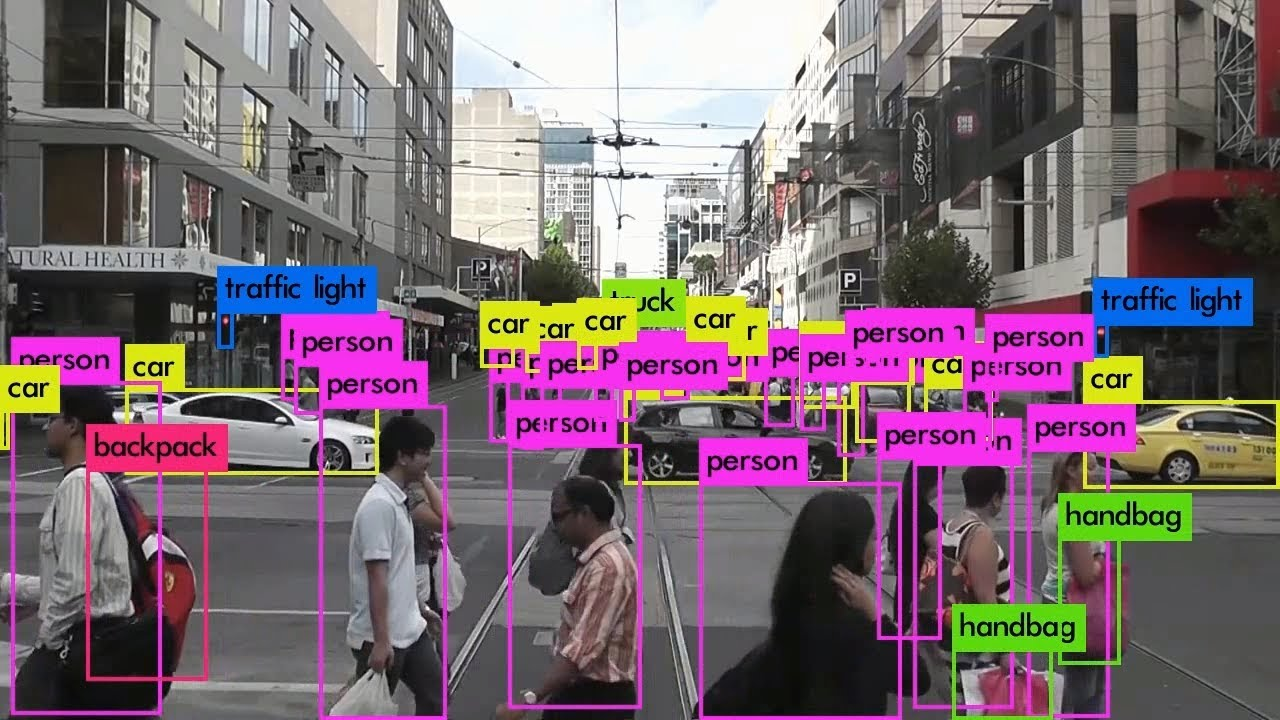
\includegraphics[width=0.8\textwidth]{images/1_1_yolov3}
    \caption{YOLO-V3 in action.}
    \label{fig:figure-yolo-v3}
\end{figure}



%**************************************************************

\section{Problem}\label{sec:problem}
The term "odometry" originated from two Greek works \emph{hodos} (meaning "journery" or "travel") and \emph{metron} (meaning "measure").
This derivation is related to the estimation of the change in a robot's pose (translation and rotation) over time.
Mobile robot use data from motion sensor to estimate their position relative to their initial location, this is called odometry.
VO is a technique used to localize a robot by using only a stream of images acquired from a single or multiple camera.
There are different ways to classify the typology of Visual Odometry:
\begin{itemize}
    \item based on the camera setup:
        \begin{itemize}
            \item Monocular VO: using only one camera;
            \item Stereo VO: using two cameras;
        \end{itemize}
    \item based on the information:
        \begin{itemize}
            \item Feature based method: which extracts the image feature points and tracks them in the image sequence;
            \item Direct method: a novel method which uses the pixel intensity in the image sequence directly as visual input.
            \item Hybrid method: which combines the two methods.
        \end{itemize}
    \item Visual inertial odometry: if a \gls{imu} is used within the VO system, it is commonly referred to as Visual inertial odometry.
\end{itemize}
We can represent the pose in different ways, for example: \textbf{euler angles}, \textbf{quaternions}, \textbf{rotation matrices} combined with \textbf{translation vectors}.

The goal is to create a \gls{nn}, using a \textbf{ResNet} to extract features from images and the \textbf{transformer} presented by Vaswani et al.~(\cite{transformer_paper}), which is able to estimate a sequence of camera poses given a sequence of images.

%**************************************************************

\section{Why transformer?}\label{sec:why-transformer}

We think that the transformer is a good candidate to solve the problem of visual odometry because it is able to learn a sequence from one domain and translate it into another sequence from another domain.
This kind of task is called sequence-to-sequence translation, e.g., machine translation.

Traditionally, this task is tackled by using recurrent neural networks (RNNs), but they have some limitations, such as the vanishing gradient problem, which makes them difficult to train.

Other VO approaches uses the CNNs, but in CNNs the features are statically weighted using pretrained weights, while in the transformer the features are dynamically weighted based on the context and receptive fields of CNNs can be limiting the performance of the whole network.
The success of the CNN derives from the fact the shared weights explicitly encode how specific identical patterns are repeated in images, this ensures the convergence also in relatively small dataset, but also limits the modelling capacity.
Meaning that CNNs can converge to a good performance also with a relatively small dataset.

Meanwhile, the vision transformers do not enforce such strict bias, so, transformer has the higher learning capacity, but it's harder to train.

So, given the high learning capacity of the transformer, its capability to adapt to various tasks and its good ability in seq2seq translation, we think that it is a good candidate to solve the problem of visual odometry.


%**************************************************************

%! Author = wxw85
%! Date = 01/08/2022

\section{Solution}\label{sec:solution}
%**************************************************************

We tried to tackle the problem by designing a deep neural network which is composed by a feature extractor, the transformer and a MLP to predict the pose.
We feed the feature extractor with a sequence of images, we tried both grey-scale and RGB images, in this way, we obtain a sequence of embeddings (both size 512 and 2048), the embedding are then fed into the transformer (both encoder-only and encoder-decoder version) and the output of the transformer is fed into the MLP to predict the sequence of poses.

\begin{figure}[H]
    \centering
    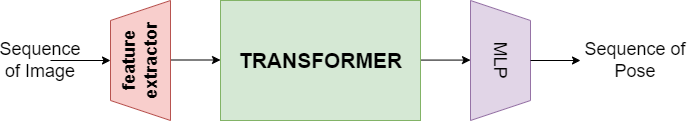
\includegraphics[width=0.8\textwidth]{images/1_4_general_solution}
    \caption{General representation of the model.}
    \label{fig:figure-1_4_solution}
\end{figure}

We use a sequence of image because the transformer model, originally designed for the machine translation, it requires as input a sequence of embeddings, then it outputs another sequence of embeddings.
For major details about the transformer, we refer to \hyperref[sec:exp-models]{\S4.1 Experiments - Models} and \hyperref[sec:models]{\S5.3 Implementation - Models}.

%**************************************************************

\section{Thesis organization}\label{sec:thesis-organization}
\begin{description}
    \item[{\hyperref[ch:introduction]{First chapter}}] introduces the general content about thesis and gives a short presentation of the topic, the problem and the solution we propose;

    \item[{\hyperref[ch:theoretical-foundations]{Second chapter}}] a deepening about the theoretical foundations used during the stage and the project;

    \item[{\hyperref[ch:datasets]{Third chapter}}] presents the datasets used during for the training and the testing of the model;

    \item[{\hyperref[ch:experiments]{Fourth chapter}}] presents the experiments did during to develop the system;

    \item[{\hyperref[ch:implementations]{Fifth chapter}}] presents the different implementations of the system;

    \item[{\hyperref[ch:final-discussions]{Sixth chapter}}] discusses about the results and possible future developments.
\end{description}
During the drafting of the essay, following typography conventions are considered:
\begin{itemize}
    \item the acronyms, abbreviations, ambiguous terms or terms not in common use are defined in the glossary, in the end of the present document;
    \item the first occurrences of the terms in the glossary are highlighted like this: \gls{word};
    \item the terms from the foreign language or jargon are highlighted like this: \emph{italics}.
\end{itemize}

%**************************************************************


    % !TEX encoding = UTF-8
% !TEX TS-program = pdflatex
% !TEX root = ../tesi.tex

%**************************************************************

\chapter{Background notions}
\label{ch:background-notions}
%**************************************************************

%**************************************************************

\section{The Prolog Language}\label{sec:the_prolog_Language}

\subsection{Brief History}\label{subsec:brief_history_prolog}
Prolog stands for \textit{PROgrammation en LOGique} and it emerged during 1970s as a way to use logic as a programming language.
The early developers of this language were Robert Kowalski, Maarten van Emden and Alain Colmelauer. The programming language, Prolog, was born of a project aimed not at producing a programming
language but at processing natural languages; in this case, French \cite{10.1145/155360.155362}. The project gave rise to a preliminary
version of Prolog at the end of 1971 and a more definitive version at the end of 1972.
Prolog gained a lot of attraction from the computing society as it was the very first logic programming language.
The language still holds considerable importance and popularity among the logic programming languages and comes with a range of commercial as well as free implementations.
\newline
Prolog is used for different kind of tasks such as:
\begin{itemize}
    \item theorem proving \cite{coelho1986automated}
    \item expert systems \cite{merritt2012building}
    \item knowledge representation \cite{gelfond2002logic}
    \item automated planning \cite{pinna2015resolving}
    \item natural language processing \cite{lally2011natural}
\end{itemize}


\subsection{Concepts}\label{subsec:concepts}
Syntax and semantics of Prolog are described in ISO standard ISO/IEC 13211. Prolog is a logic programming language; 
this means that it is used to describe known facts and relationships about a problem and less about prescribing
the sequence of steps taken by a computer to solve the problem.
When a computer is programmed in Prolog, the actual way the computer carries out the computation is specified
partially by the logic declarative semantics of Prolog, partly by what new facts can be inferred from the given ones,
and only partly by explicit control information supplied by the programmer.
\newline\newline
Prolog is used to solve problems which involve objects and relations among them.
The main features of the programming language are:
\begin{itemize}
    \item specifyng some \textit{facts} about some objects and their relationships
    \item defining some \textit{rules} about object and their relationships
    \item asking \textit{questions} about objects and their relationships
\end{itemize}

Prolog programs are built from terms. A term is either a constant, a variable or a structure.\newline
\subsubsection{Constants}\label{subsubsec:constants}
A constant is a sequence of characters which denotes a specific object or relationship. A constant can be an atom or a number.
All constants begin with a lower case letter.\newline\newline
\textbf{Example}\newline\newline
\textit{a} is an atom\newline
\textit{12} is a number

\subsubsection{Variables}\label{subsubsec:variables}
A variable looks like an atom except it has a name beginning with capital letter or underline signed.
A variable should be thought of as standing for some objects we are unable or unwilling to name at the time we write the program.\newline\newline
\textbf{Example}\newline\newline
\textit{X} and \textit{Answer} are valid names for variables

\subsubsection{Structures}\label{subsubsec:structure}
A structure is a collection of other objects called \textit{components}. Structures help to organize the data in a program because
they permit a group of related information to be treated as a single object instead of separate entities.
A structure is written in Prolog by specifying its \textit{functor} and its \textit{components}. The coponents are enclosed in round brackets
and separated by commas. The functor is written just before the opening round brackets.\newline\newline
\textbf{Example}\newline\newline
owns(john,book) is a structure having owns as functor and, john and book as components
\subsubsection{Facts}\label{subsubsec:facts}
A fact is a relation among objects which are all \textit{ground}. This means that a fact is a \textit{structure} which does not contain any variables among its components.
A fact is written as a structure followed by a dot (.). The names of the objects that are enclosed within the round brackets in each fact are called \textit{arguments}.
The name of the relationship which comes just before the round brackets is called \textit{predicate}.\newline\newline
\textbf{Example}\newline\newline
\textit{king(john,france)}. is a fact

\subsubsection{Rules}\label{subsubsec:rules}
A rule is a disjunction of predicates, where at most one is not negated, written in the following way:
\[ Head :- Body.\]
where Head is a predicate, Body is a conjunction of predicates and the symbol ":-" means that the body implies the head. This kind of structure is called Horn clause.
A Prolog program can be seen as a list (because order matters) of Horn clauses called \textit{theory}.
Facts could be seen as Rules having Body equals to true.
Rules are used to describe some complex relations among objects of the domain of discourse and differently from facts can contain variables.\newline\newline
\textbf{Example}\label{subsubsec:rules}\newline\newline
motherOf(X,Y) :- parentOf(X,Y),female(X).\newline\newline
The aforementioned description of Prolog language has been adapted from \cite{Clocksin1987ProgrammingIP}.

\subsubsection{Unification}\label{subsubsec:Unification}
A substitution is a function which associates a variable to a given term. The most general unifier (m.g.u.) is the substitution which allows to transform two predicates making them equals
such that all other substitutions can be obtained through a composition with this one.
The unification is a process whereby two structures are made equals via substitution and it is used several times during the Prolog resolution process. 

\subsubsection{Resolution}\label{subsubsec:resolution}
The resolution in Prolog happens in the following way:the interpreter tries to verify whether a conjunction of predicates (the goal) provided by the user can be derived
from the current program or not and in the case it could, it provides a computed answer substitution (c.a.s.) which is a set of substitutions which allow to make true the user's goal.\newline
Prolog resolution process is called SLD (Selective Linear Definite clause resolution) and works as follows:\newline
SLD resolution implicitly defines a search tree of alternative computations, in which the initial goal clause is associated with the root of the tree. For every node in the tree and for every definite clause in the program whose positive literal unifies with the selected literal in the goal clause associated with the node, there is a child node associated with the goal clause obtained by SLD resolution.
A leaf node, which has no children, is a success node if its associated goal clause is the empty clause. It is a failure node if its associated goal clause is non-empty but its selected literal unifies with no positive literal of definite clauses in the program.
SLD resolution is non-deterministic in the sense that it does not determine the search strategy for exploring the search tree. Prolog searches the tree depth-first, one branch at a time, using backtracking when it encounters a failure node. Depth-first search is very efficient in its use of computing resources, but is incomplete if the search space contains infinite branches and the search strategy searches these in preference to finite branches: the computation does not terminate.
The SLD resolution search space is an or-tree, in which different branches represent alternative computations.\cite{Gallier1985LogicFC}

\subsection{2p-Kt}\label{subsec:2p_kt}

2p-Kt is a general, extensible, and interoperable ecosystem for logic programming and symbolic AI written in Kotlin which supports the Prolog ISO standard.\newline
\begin{figure}[h]
    \centering
    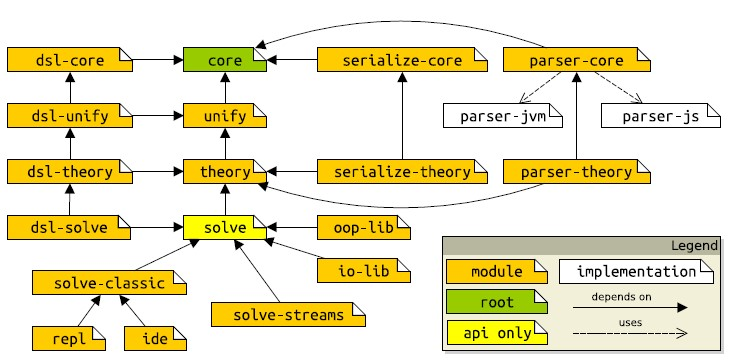
\includegraphics[width=0.70\textwidth]{images/2p_kt.jpg}
    \caption{2P-Kt project map. LP functionalities are partitioned into some loosely-coupled and incrementally-dependent modules.}
    \label{fig:2p_kt}
\end{figure}
2p-kt is the evolution of another project called tuProlog \cite{CIATTO2021100817}. To support reusability 2p-Kt is divided into several modules described as follows:
\begin{itemize}
    \item \textbf{:core}: exposes data structures for knowledge representation via terms and clauses, other than methods supporting their manipulation
    \item \textbf{:unify}: used to compare and manipulate logic terms through logic unification
    \item \textbf{:theory}: in-memory storage of clauses into ordered (e.g. queues) or unordered (e.g. multisets) data structures, and their efficient retrieval via pattern-matching
    \item \textbf{:serialize-* and :parser-*}: used to perform ancillary operations such as serialization and parsing
    \item \textbf{:solve}: aspects which are orthogonal w.r.t. any particular resolution strategy—e.g. errors management, extensibility via libraries, I/O, etc
    \item \textbf{:solve-*}: modules which implement a specific resolution strategy
    \item \textbf{:repl and :ide}: provide CLI and GUI
\end{itemize}
The structure of the project can be seen in figure \ref{fig:2p_kt}.\newline
2p-Kt provides a well-grounded technological basis for implementing/experimenting/extending the many solutions proposed in the literature—e.g., abductive
inference, rule induction, probabilistic reasoning and labelled LP.

%**************************************************************

\section{Constraint Programming}\label{sec:constraint_programming}

Constraint Programming is a paradigm for solvig combinatorial problems where
different constraints are imposed on feasible solutions for different decision variables, each having
its own domain. Constraints are relations among variables which limit the values decision variables
can assume in feasible solutions \cite{10.5555/2843512}

\subsection{Brief History}\label{subsec:brief_history_cp}
In artificial intelligence interest in constraint satisfaction developed in two streams. In
some sense a common ancestor of both streams is Ivan Sutherland’s groundbreaking 1963
MIT Ph.D. thesis, “Sketchpad: A man-machine graphical communication system”.
In one stream, the versatility of constraints led to applications in a variety of domains,
and associated programming languages and systems. This stream we can call the language
stream. In 1964 Wilkes proposed that algebraic equations be allowed as constraint statements
in procedural Algol-like programming languages, with relaxation used to satisfy the
constraints. Around 1967, Elcock developed a declarative language, Absys, based on
the manipulation of equational constraints.

\subsection{Concepts}\label{subsec:concepts_cp}

There are mainly two types of constraint programming problems: CSP (Constraint Satisfaction Problem) and COP (Constraint Optimization Problem).\newline\newline
A \textit{constraint satisfaction problem} (CSP) involves finding solutions to a constraint network,
that is, assignments of values to its variables that satisfy all its constraints. Constraints
specify combinations of values that given subsets of variables are allowed to take.\newline
A constraint can be specified extensionally by the list of its satisfying tuples, or intensionally
by a formula that is the characteristic function of the constraint.\newline\newline
A \textit{constraint optimization problem} (COP) is basically the same as a CSP but in addition to the aforementioned constraints there is another one
which consists of finding a solution which minimizes or maximizes a certain function.


\subsection{Constraint Logic Programming}\label{subsec:clp}

\textit{Constraint Logic Programming} (CLP) began as a natural merger of two declarative paradigms: constraint solving and logic programming \cite{JAFFAR1994503}.\newline
Viewing the subject rather broadly, constraint logic programming can be said to involve the
incorporation of constraints and constraint “solving” methods in a logic-based language.
This characterization suggests the possibility of many interesting languages, based on different constraints and different logics. However, to this point, work on CLP has almost
exclusively been devoted to languages based on Horn clauses.\newline
Prolog can be said to be a CLP language where the constraints are equations over the
algebra of terms (also called the algebra of finite trees, or the Herbrand domain). The equations are implicit in the use of unification.

\subsection{SWI Prolog - CLP libraries}\label{subsec:clp_swi}

SWI-Prolog is an implementation of the Prolog language which is strong in education because it is free and portable, but also because of its compatibility with textbooks and its easy-to-use environment.\newline
SWI-Prolog is used as an embedded language where it serves as a small rule subsystem in a large application. The syntax and set of built-in predicates is based on the ISO standard \cite{SWI-Prolog}.

\subsubsection{CLP(X) libraries}\label{subsubsec:clp_libraries}
CLP(X) stands for constraint logic programming over the domain X. Plain Prolog can be regarded as CLP(H), where H stands for Herbrand terms.\newline
SWI Prolog supports:\newline
\begin{itemize}
    \item \textbf{CLP(FD)} for integers
    \item \textbf{CLP(B)} for boolean variables
    \item \textbf{CLP(Q)} for rational numbers
    \item \textbf{CLP(R)} for floating point numbers
\end{itemize}

All constraints contained in these libraries will be deeply explained
in chapter \ref{ch:clp_2p_kt}.\newline\newline
\textbf{CLP(FD)} has two main usages:
\begin{itemize}
    \item declarative integer arithmetics
    \item solving combinatorial problems such as planning, scheduling and allocation tasks
\end{itemize}
The predicate of this library can be classified as:
\begin{itemize}
    \item \textit{arithmetic constraints}
    \item \textit{membership constraints}
    \item \textit{enumeration predicates}
    \item \textit{combinatorial constraints}
    \item \textit{reification predicates}
    \item \textit{reflection predicates}
\end{itemize}

Practical usage of these constraints can be found in \cite{Triska12}.\newline\newline
\textbf{CLP(Q) and CLP(R)} share basically the same constraints except for \textit{bb\_inf}
constraint which is used to find a minimum in the case of mixed integer programming.\newline\newline
\textbf{CLP(B)} can be used to model and solve combinatorial problems such as verification, allocation and covering tasks.
Benchmarks and usage examples of this library are available from \cite{Triska2016} and \cite{Triska2018}.


%**************************************************************

    % !TEX encoding = UTF-8
% !TEX TS-program = pdflatex
% !TEX root = ../tesi.tex

%**************************************************************
\chapter{CLP in 2p-Kt}
\label{ch:clp_2p_kt}

%%**************************************************************
%
\section{Requirements}\label{sec:Requirements}

As described in section \ref{subsec:2p_kt}, 2P-Kt is an exensible framework with different mechanisms
which could be used to add to the standard Prolog other features; in this case we deal with Constraint Logic Programing (CLP).\newline
The main purpose of the following project is to implement CLP libraries in 2P-Kt having the following requirements:
\begin{itemize}
    \item the interface of the predicates exposed by the libraries must be as close as possible to the one used by SWI Prolog for CLP
    \item there are not strict requirements about how to implement libraries but a good solution would exploit on existing components in 2P-kt
    \item the different libraries could contain different predicates wrt SWI Prolog only if it is not possible to find another solution which is compatible with the current framework
\end{itemize}


%
%%**************************************************************
%
\section{Design}\label{sec:design}

\subsection{Common aspects}\label{subsec:common_aspects}
Four different libraries have been realized:
\begin{itemize}
    \item \textbf{clp-core} for basic functionality of the other libraries
    \item \textbf{clpfd} for integer variables
    \item \textbf{clpqr} for rational and real variables
    \item \textbf{clpb} for boolean variables
\end{itemize}
\textbf{clpqr} contains basically the predicates of \textbf{clpq} and \textbf{clpr} because there
is any distinction between rational and reals in 2P-Kt.\newline

Libraries will be described in the following sections highlighting common and/or different aspects with respect to the SWI Prolog counterpart.

\subsection{Constraint Logic Programming over Finite Domains}\label{subsec:clpfd}
For a better explaination predicates will be divided in groups as described in section \ref{subsubsec:clp_libraries}.

\subsubsection{Arithmetic Constraints}\label{subsubsec:arithmetic_constraints}

All constraints supported by SWI Prolog are supported; constraints are the followings:\newpage
\begin{center}
    \begin{table}
        \begin{tabular}{||c c ||} 
        \hline
        Constraint & Explaination \\ [0.5ex] 
        \hline\hline
        Expr1 \#= Expr2	& Expr1 equals Expr2 \\ 
        \hline
        Expr1 \#\= Expr2 & Expr1 is not equal to Expr2 \\
        \hline
        Expr1 \#>= Expr2 & Expr1 is greater than or equal to Expr2\\
        \hline
        Expr1 \#=< Expr2 & Expr1 is less than or equal to Expr2 \\
        \hline
        Expr1 \#> Expr2	& Expr1 is greater than Expr2 \\
        \hline
        Expr1 \#< Expr2	& Expr1 is less than Expr2 \\
        \hline
        \end{tabular}
        \label{table:arithmetic_constraints}
        \caption{Arithmetic constraints in clpfd}
    \end{table}    
\end{center}

\begin{center}
    \begin{table}
        \begin{tabular}{||c c ||} 
        \hline
        Expression & Explaination \\ [0.5ex] 
        \hline\hline
        integer	& Given value \\ 
        \hline
        variable & Unknown integer \\
        \hline
        -Expr & Unary minus\\
        \hline
        Expr + Expr	 & Addition \\
        \hline
        Expr * Expr	& Multiplication \\
        \hline
        Expr - Expr	& Subtraction \\
        \hline
        Expr \^ Expr& Exponentiation \\
        \hline
        min(Expr,Expr) & Minimum of two expressions \\
        \hline
        max(Expr,Expr) & Maximum of two expressions \\
        \hline
        Expr mod Expr & Modulo induced by floored division \\
        \hline
        abs(Expr) & Absolute value \\
        \hline
        Expr div Expr & Floored integer division \\
        \hline
        \end{tabular}
        \label{table:expressions_clp}
        \caption{Arithmetic expressions in clpfd}
    \end{table}    
\end{center}

\textit{Expr1} and \textit{Expr2} are \textbf{arithmetic expressions}.
\textit{Expr rem Expr} and \textit{Expr // Expr} are not supported. \textit{rem} is modulo induced by truncated division
whereas \textit{//} is truncated integer division.

\subsubsection{Membership Constraints}\label{subsubsec:Membership}

These constraints are used to specify the admissible domains of variables.\newline
The predicates are:\newline
\begin{itemize}
    \item \textbf{Var in Domain}: Var is an element of Domain; Domain is either an integer or an interval (expressed as Lower..Upper)
    \item \textbf{Vars in Domain}: The variables in the list Vars are elements of Domain
\end{itemize}

It is not current supported \textit{\/} (union of domains) as expression for building a domain.

\subsubsection{Enumeration predicates}\label{subsubsec:enumeration}

These predicates are used to customize the search to find a feasible assignments of all variables such that all constraints are satisfied.\newline
The predicates are \textbf{labeling/2 and label/1}.\newline\newline
\textbf{labeling(Options, Vars)}\newline\newline
Assign a value to each variable in Vars; Options is a list of options that let exhibit some control over the search process. Several categories of options exist:\newline
\begin{itemize}
    \item \textbf{variable selection strategy}: it can the order in which the variable occurs (\textit{leftmost}, it is the default), the leftmost variable with smallest domain (\textit{ff}), the variables with smallest domains, the leftmost one participating in most constraints (\textit{ffc}), the leftmost variable whose lower bound is the lowest (\textit{min}) or the leftmost variable whose upper bound is the highest (\textit{max})
    \item \textbf{value order}: elements of the chosen variable's domain in ascending order (\textit{up}, it is the default) or domain elements in descending order (\textit{down})
    \item \textbf{branching strategy}: For each variable X, a choice is made between X = V and X \#\= V, where V is determined by the value ordering options. This option is called \textit{step}, it is the default and the only branching option supported
\end{itemize}

At most one option of each category can be specified, and an option must not occur repeatedly.\newline
The order of solutions can be influenced with:\newline
\begin{itemize}
    \item min(Expr)
    \item max(Expr)
\end{itemize}

This generates solutions in ascending/descending order with respect to the evaluation of the arithmetic expression Expr. Labeling Vars must make Expr ground. If several such options are specified, they are interpreted from left to right.\newline
This predicate does not support as options the following branching strategies:\newline
\begin{itemize}
    \item \textit{enum}: For each variable X, a choice is made between X = V\_1, X = V\_2 etc., for all values V\_i of the domain of X. The order is determined by the value ordering options.
    \item \textit{bisect}: For each variable X, a choice is made between X \#=< M and X \#> M, where M is the midpoint of the domain of X.
\end{itemize}
\textbf{label(Vars)}\newline\newline
Equivalent to labeling([], Vars).

\subsubsection{Global constraints}\label{subsubsec:global_constraints}
A global constraint expresses a relation that involves many variables at once. The implemented constraints are the followings:
\begin{itemize}
    \item \textbf{all\_distinct(Vars)}: True iff Vars are pairwise distinct
    \item \textbf{sum(Vars, Rel, Expr)}: The sum of elements of the list Vars is in relation Rel to Expr. Rel is one of \#=, \#\=, \#<, \#>, \#=< or \#>=
    \item \textbf{scalar\_product(Cs, Vs, Rel, Expr)}: True iff the scalar product of Cs and Vs is in relation Rel to Expr. Cs is a list of integers, Vs is a list of variables and integers. Rel is \#=, \#\=, \#<, \#>, \#=< or \#>=
    \item \textbf{lex\_chain(Lists)}: Lists are lexicographically non-decreasing
    \item \textbf{tuples\_in(Tuples, Relation)}: True iff all Tuples are elements of Relation. Each element of the list Tuples is a list of integers or finite domain variables. Relation is a list of lists of integers
    \item \textbf{serialized(Starts, Durations)}: Describes a set of non-overlapping tasks. Starts = $[S_1,...,S_n]$, is a list of variables or integers, Durations = $[D_1,...,D_n]$ is a list of non-negative integers. Constrains Starts and Durations to denote a set of non-overlapping tasks, i.e.: S\_i + D\_i =< S\_j or S\_j + D\_j =< S\_i for all 1 =< i < j =< n
    \item \textbf{element(N, Vs, V)}: The N-th element of the list of finite domain variables Vs is V
    \item \textbf{global\_cardinality(Vs, Pairs)}: Global Cardinality constraint. Vs is a list of finite domain variables, Pairs is a list of Key-Num pairs, where Key is an integer and Num is a finite domain variable. The constraint holds iff each V in Vs is equal to some key, and for each Key-Num pair in Pairs, the number of occurrences of Key in Vs is Num
    \item \textbf{circuit(Vs)}: True iff the list Vs of finite domain variables induces a Hamiltonian circuit. The k-th element of Vs denotes the successor of node k
    \item \textbf{cumulative(Tasks, Options)}: Schedule with a limited resource. Tasks is a list of tasks, each of the form task(S\_i, D\_i, E\_i, C\_i, T\_i). S\_i denotes the start time, D\_i the positive duration, E\_i the end time, C\_i the non-negative resource consumption, and T\_i the task identifier. Each of these arguments must be a finite domain variable with bounded domain, or an integer. The constraint holds iff at each time slot during the start and end of each task, the total resource consumption of all tasks running at that time does not exceed the global resource limit. Options is a list of options. Currently, the only supported option is \textit{limit(L)} which is the global resource limit
    \item \textbf{cumulative(Tasks)}: Like the previous one but with \textit{L = 1}
    \item \textbf{disjoint2(Rectangles)}: True iff Rectangles are not overlapping. Rectangles is a list of terms of the form F(X\_i, W\_i, Y\_i, H\_i), where F is any functor, and the arguments are finite domain variables or integers that denote, respectively, the X coordinate, width, Y coordinate and height of each rectangle.
    \item \textbf{chain(Zs, Relation)}: Zs form a chain with respect to Relation. Zs is a list of finite domain variables that are a chain with respect to the partial order Relation, in the order they appear in the list. Relation must be \#=, \#=<, \#>=, \#< or \#>
\end{itemize}
\textbf{Notes}\newline\newline
Wrt global constraints provided by CLP(FD) library of SWI Prolog the following aspects are different:
\begin{itemize}
    \item the index of the predicate \textbf{circuit/1} starts from 1 and not from 0 for implementation issues
    \item the predicate \textbf{all\_different/1} has not been supported because it has the same usage of \textbf{all\_distinct} but it has a weaker propagation which cannot be simulated
    \item predicates \textbf{automaton/3} and \textbf{automaton/8} have not been implemented because of the fact that these predicates are rarely used and tedious to use
    \item the predicate \textbf{global\_cardinality/3} can be used but actually it throws an exception because the Option parameter cannot be supported
\end{itemize}

\subsubsection{Reification Predicates}\label{subsubsec:reification}
All relational constraints discussed in \ref{subsubsec:arithmetic_constraints} can be reified.
This means that their truth value is itself turned into a clpfd variable, so that it is possible to reason about whether a constraint holds or not. These predicates are reifiable themselves.
\begin{itemize}
    \item \textbf{\#\ Q}: Q does not hold
    \item \textbf{P \#<==> Q}: P and Q are equivalent
    \item \textbf{P \#==> Q}: P implies Q
    \item \textbf{P \#<== Q}: Q implies P
    \item \textbf{P \#/\ Q}: P and Q hold
    \item \textbf{P \#\/ Q}: P or Q hold
    \item \textbf{P \#\ Q}: Either P holds or Q holds, but not both
    \item \textbf{zcompare(Order, A, B)}: reify an arithmetic comparison of two integers
\end{itemize}

\subsubsection{Reflection Predicates}\label{subsubsec:reflection}
Reflection predicates let obtain, in a well-defined way, information that is normally internal to this library. Predicates are:
\begin{itemize}
    \item \textbf{fd\_var(Var)}: True iff Var is a clpfd variable
    \item \textbf{fd\_inf(Var, Inf)}: Inf is the infimum of the current domain of Var
    \item \textbf{fd\_sup(Var, Sup)}: Sup is the supremum of the current domain of Var
    \item \textbf{fd\_size(Var, Size)}: Reflect the current size of a domain. Size is the number of elements of the current domain of Var
    \item \textbf{fd\_dom(Var, Dom)}: Dom is the current domain (see \ref{subsubsec:enumeration}) of Var
    \item \textbf{fd\_degree(Var, Degree)}: Degree is the number of constraints currently attached to Var
\end{itemize}

\subsection{Constraint Logic Programming over Rationals and Reals}\label{subsec:clpqr}
This library is very different from the previous one because variable definitions and constraints can be stated in the same structure. The main predicate is
\textbf{\{\}(Constraints)} which allows to add the constraints given by Constraints to the constraint store.\newline
\textit{Constraints} can be defined using the following grammar:

\begin{figure}[h]
    \centering
    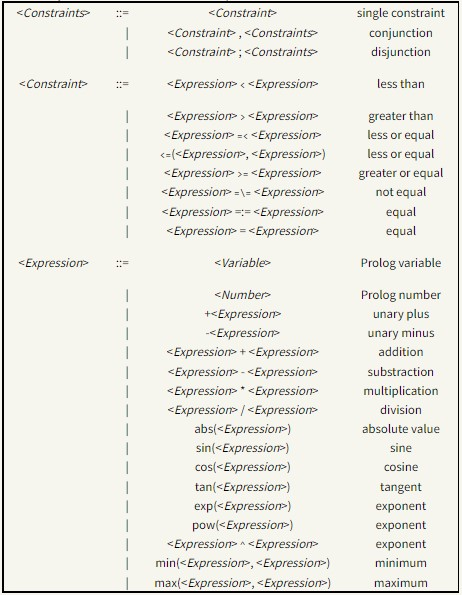
\includegraphics[width=0.70\textwidth]{images/bnf_constraints.jpg}
    \caption{clpqr constraints BNF}
    \label{fig:bnf_constraints}
\end{figure}

All constraints are supported except for \textit{<Expression> =\= <Expression>} (not equal).
This libraries contain also the following predicates:
\begin{itemize}
    \item \textbf{entailed(Constraint)}: Succeeds if Constraint is necessarily true within the current constraint store. This means that adding the negation of the constraint to the store results in failure
    \item \textbf{inf(Expression, Inf)}: Computes the infimum of Expression within the current state of the constraint store and returns that infimum in Inf. This predicate does not change the constraint store
    \item \textbf{sup(Expression, Sup)}: Computes the supremum of Expression within the current state of the constraint store and returns that supremum in Sup. This predicate does not change the constraint store
    \item \textbf{minimize(Expression)}: Minimizes Expression within the current constraint store. This is the same as computing the infimum and equating the expression to that infimum
    \item \textbf{maximize(Expression)}: Maximizes Expression within the current constraint store. This is the same as computing the supremum and equating the expression to that supremum
    \item \textbf{bb\_inf(Ints, Expression, Inf, Vertex, Eps)}: It computes the infimum of Expression within the current constraint store, with the additional constraint that in that infimum, all variables in Ints have integral values. Vertex will contain the values of Ints in the infimum. Eps denotes how much a value may differ from an integer to be considered an integer
    \item \textbf{bb\_inf(Ints, Expression, Inf, Vertex)}: it behaves as the previous one but not use an error margin
    \item \textbf{bb\_inf(Ints, Expression, Inf)}: as the previous one but without returning the values of the integers
    \item \textbf{dump(Target, Newvars, CodedAnswer)}: Returns the constraints on Target in the list CodedAnswer where all variables of Target have been replaced by NewVars. This operation does not change the constraint store
\end{itemize}
\textbf{Notes}\newline\newline
Eps of the predicate \textbf{bb\_inf/5} cannot be fully supported, the only admissible value is 0.

\subsection{Constraint Logic Programming over Boolean Variables}\label{subsec:clpb}

All predicates of this library are based on the concept of \textit{boolean expression}. A \textit{boolean expression} is one of:
\begin{center}
    \begin{table}
        \begin{tabular}{||c c ||} 
        \hline
        Expression & Explaination \\ [0.5ex] 
        \hline\hline
        0 & false \\
        \hline
        1 & true \\ 
        \hline
        variable & unknown truth value \\
        \hline
        ~ Expr & logical NOT\\
        \hline
        Expr + Expr & logical OR \\
        \hline
        Expr * Expr & logical AND \\
        \hline
        Expr \# Expr & exclusive OR \\
        \hline
        Expr =:= Expr & equality \\
        \hline
        Expr =\= Expr & disequality (same as \#) \\
        \hline
        Expr =< Expr & less or equal (implication) \\
        \hline
        Expr >= Expr & greater or equal \\
        \hline
        Expr < Expr	& less than\\
        \hline
        Expr > Expr	& greater than \\
        \hline
        +(Exprs) & n-fold disjunction \\
        \hline
        *(Exprs) & n-fold conjunction \\
        \hline
        \end{tabular}
        \label{table:boolean_expressions}
        \caption{Admissible boolean expressions in clpb}
    \end{table}    
\end{center}

Supported predicates are:
\begin{itemize}
    \item \textbf{sat(Expr)}: True iff the Boolean expression Expr is satisfiable
    \item \textbf{taut(Expr, T)}: If Expr is a tautology with respect to the posted constraints, succeeds with T = 1. If Expr cannot be satisfied, succeeds with T = 0. Otherwise, it fails
    \item \textbf{labeling(Vs)}: Assigns truth values to the variables Vs such that all constraints are satisfied
    \item \textbf{sat\_count(Expr, Count)}: Count the number of admissible assignments. Count is the number of different assignments of truth values to the variables in the Boolean expression Expr, such that Expr is true and all posted constraints are satisfiable
    \item \textbf{weighted\_maximum(Weights, Vs, Maximum)}: Enumerate weighted optima over admissible assignments. Maximize a linear objective function over Boolean variables Vs with integer coefficients Weights. This predicate assigns 0 and 1 to the variables in Vs such that all stated constraints are satisfied, and Maximum is the maximum of $sum(Weight_i*V_i)$ over all admissible assignments
    \item \textbf{random\_labeling(Seed, Vs)}: Select a single random solution. An admissible assignment of truth values to the Boolean variables in Vs is chosen in such a way that each admissible assignment is equally likely. Seed is an integer, used as the initial seed for the random number generator
\end{itemize}



%
%%**************************************************************
\section{Implementation}\label{sec:Implementation}

The aforementioned libraries have been implemented in 2P-Kt using the following interfaces and classes:
\begin{itemize}
    \item \textbf{PrimitiveWrapper}: it is an abstract class which allows to define a predicate which is not unified as usual but it executes some code producing some
    side effect on the actual substitution. This class reifies the generator concept described in \cite{10.1007/978-3-030-75775-5_27}
    where the solver can be seen as a stream consumer allowing it to get a stream of solutions interacting with a primitive mechanism (the generator)
    which can be seen by the solver as an ordinary build-in predicate denoted by its own \textit{signature} and \textit{arity}. The PrimitiveWrapper has been used to define most of predicates contained in the libraries.
    \item \textbf{RuleWrapper}: it is an abstract class which allows to define a Prolog \textit{Rule}. This class is useful to avoid
    repeated code because it allows to define some predicates in terms of other existing ones.
    \item \textbf{Library}: it is an interface which has been implemented to group together different predicates implementations which
    can be either \textit{PrimitiveWrapper} or \textit{RuleWrapper}
    \item \textbf{durable CustomData}: it is a map from String to Any which allows to store data during the resolution process. It has been used to store the
    model containing all variables and constraints of the problem
    \item \textbf{DefaultTermVisitor}: this abstract class is used to realize the visitor pattern \cite{gamma1994design} and it has been
    extensively used for different tasks such as evaluation of expressions, generation of arithmetic expressions and all other tasks related to perform different operation wrt the type of the term
\end{itemize}


The actual implementation of all constraints have been realized exploiting on the Choco Library \cite{Prud'homme2022}. This library has been chosen for different reasons:
\begin{itemize}
    \item it is written in Java and can be easily used with Kotlin language
    \item wrt other similar libraries (e.g. OR Tools \cite{ortools} or JaCoP \cite{Kuchcinski2013JaCoPJ}) it simplifies the composition of expressions for the creation of new variables or constraints
    \item well documented and with an active community to get support in case of doubts or problems
\end{itemize}

Choco Library cannot be directly mapped with SWI Prolog CLP(X) libraries
because these these libraries belong to a different paradigms. For this reason the mapping was not immediate but
sometimes different approaches have been used to solve these issues.\newline\newline
Following the main mapping choices divided by Library

\subsection{Constraint Logic Programming over Finite Domains}\label{map_clpfd}








%
%%**************************************************************
\section{Case study}\label{sec:case_study}

The aforementioned \textbf{clpfd} library has been used to realize a real case study called "SchoolTimetable".
This case study involves both Multi-Agent systems and Constraint Programming technologies.\newline\newline
Multi-Agent Systems (MAS) is an extension of the agent technology where a group of loosely connected autonomous agents act in an environment to achieve a common goal. This is done either by cooperating or competing, sharing or not sharing knowledge with each other \cite{inbook}.
Agent-oriented programming is a paradigm which is based on the concept of software agents. Several definitions have been provided, one of the most used is described in \cite{10.5555/1695886} and claims that an agent is a computer system that is situated in some environment,
and that is capable of autonomous action in this environment in order
to meet its design objectives.\newline\newline
The problem consists of finding a school timetable for each professor of a school such that different constraints related to different aspects of the problem are respected,
and trying to satisfy all preferences of each professor as much as possible.\newline\newline
Italian schools have a person (usually a professor) who is responsible for the creation of an overall timetable where for each day of the week and for each hour,
a professor must be assigned to a class according to the hours that must spend in each class as described by school regulation. This task is difficult and time-demanding because it is subjected to different constraints related to professors and classes where they teach.
Sometimes it can also happen that a professor asks for a lesson change due to own commitments or needs and this entails finding a lesson change which keeps still valid the aforementioned constraints.\newline
More in details the requirements are the followings:
\begin{itemize}
    \item There is a person, responsible for the creation of the timetable of each professor (time-scheduler), who receives from school direction all information to perform the aforementioned task
    \item After the creation of timetables, the time-scheduler must send to each professor the corresponding timetable
    \item Each professor must spend exactly in each class a number of hours described by the school regulation according to the number and type of class where the teaching happens
    \item Each professor must have a free day during the school week
    \item In the same class cannot be more than one professor per hour (this requirement has been imposed to simplify particular cases, e.g. laboratories, where two professor teach in the same class)
    \item Each professor can have own preferences related to the lessons in which he/she would rather not teach 
    \item Each professor can begin a negotiation trying to satisfy own preferences, mediated by the time-scheduler   
\end{itemize}

\subsection{Implementation}\label{subsec:implementation_case_study}
The system has been implemented using a MAS framework called Jade \cite{10.1007/3-540-44631-1_7}.
Jade (Java Agent DEvelopment framework) is a MAS framework developed in Java which supports the notion of agent. It has been used to simulate the time-scheduler and the professors as agents which interact in the same environment.\newline
To implement the Constraint Programming new features have been added to \textbf{clpfd} library which are not supported in SWI Prolog:
\begin{itemize}
    \item \textbf{all\_distinct\_except\_0}: a predicate which states that all variables must be different except for 0 which can occur with repetitions
    \item \textbf{tuples\_in} with reification: reification operators supported only relational predicates or reified predicate themselves. Now this predicate is also suported
\end{itemize}

\subsection{Design}\label{subsec:design}

Several design choices have been taken and will be explained according to the kind of paradigm they
affect

\subsubsection{Multi-Agent Systems (MAS)}\label{subsubsec:mas}
There are two types of agents: \textbf{TimeScheduler} and \textbf{Professor}.\newline
\textbf{TimeScheduler} agent has in its own state all information related to the amount of hours each professor must spend in each class and knows the Agent Identifier (AID) of each \textbf{Professor} agent. Moreover, it uses the Directory Facilitator (DF) agent to register its own service of negotiation mediator.\newline
The \textbf{TimesScheduler} is responsible for the following tasks:
\begin{itemize}
    \item creation of timetables
    \item communication of timetables to each professor
    \item mediation of negotiation among professors for the satisfaction of their preferences
\end{itemize}
These tasks are accomplished with the following Behaviors:
\begin{itemize}
    \item \textbf{TimetableBehaviour}: it produces the different timetables, save and send each of them to the corresponding professor
    \item \textbf{WaitProposalBehavior}: it waits for a cfp message from a professor to begin a negotiation
    \item \textbf{MediationBehaviour}: it mediates negotiation among professors for preferences satisfaction
\end{itemize}
\textbf{Professor} agent is an abstract class which is used to keep a common architecture for all professors which differ only for their preferences.\newline
\textbf{Professor} agents perform the following tasks:
\begin{itemize}
    \item receive the timetable
    \item try to satisfy own preferences
    \item decide whether to accept a lesson change or not
\end{itemize}
In order to do these tasks they have the following Behaviours:
\begin{itemize}
    \item \textbf{TimetableBehaviour}: it receives the timetable and save it
    \item \textbf{PreferenceBehaviour}: for a specific number of times it tries to satisfy unsatisfied preferences
    \item \textbf{NegotiationBehaviour}: it starts a negotiation for a specific unsatisfied preference
    \item \textbf{WaitProposalBehavior}: it waits for a request message from the timescheduler corresponding to a change proposal and manages it with a CandidateBehaviour
    \item \textbf{CandidateBehaviour}: it replies to the proposal of a specific lesson change
\end{itemize}
\textbf{Professor} agents, after receiving the timetable, register the classes where they teach as services interacting with the DF agent. This is done because when the \textbf{Timescheduler} agent will receive a lesson change request, it will look for all professors who teach in the same class where the proposed change happens.\newline
Another important design choice is related to the following aspect: when a professor asks for a lesson change, it must be sure that before the end of the negotiation, the current lesson cannot be available to other incoming requests. To do this, in the \textbf{NegotiationBehaviour} the current lesson is added to a set of locked lessons. In this way if another professors ask him/her to change this lesson, the request will not be able to be satisfied.
\subsubsection{Communication among agents}


\begin{figure}[h]
    \centering
    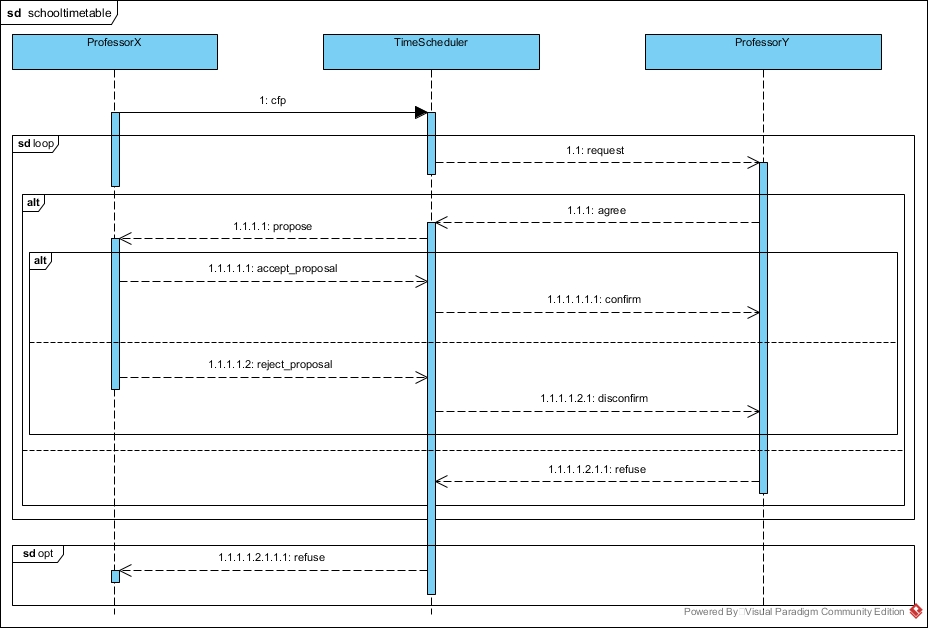
\includegraphics[width=0.60\textwidth]{images/sequence_diagram.jpg}
    \caption{Sequence Diagram of the interaction among agents}
    \label{fig:seq_diagram}
\end{figure}
The interaction among time-scheduler and professors can be explained as follows (as shown in figure \ref{fig:seq_diagram}):\newline
when a professor wants to change an own lesson in order to satisfy a preference, a call-for-proposal (cfp) message is sent to the time-scheduler to begin the negotiation.
The time-scheduler will retrieve the list of all professors who teach in the same class of the proposer's lesson. To have a reasonable change it is also important to consider that for each candidate professor and for each candidate lesson:
\begin{itemize}
    \item the proposer must be free during a candidate lesson
    \item the candidate professor must be free during the lesson the time-scheduler wants to propose.
    \item the proposer's lesson cannot be in the free day of the candidate professor and the candidate lesson cannot be in the free day of the proposer professor
\end{itemize}
Following these criteria, the time-scheduler will realize a list of pair professor-lesson and will try to satisfy the proposer's request with one of them.
The time-scheduler sends to the candidate professor a proposal and this proposal can be accepted according to two criteria:
\begin{itemize}
    \item the proposed lesson is not one of own preferences
    \item the lesson to give must not be in the locked preferences
\end{itemize}
If these criteria are met, the candidate professor replies with an agree message otherwise refuses.
If the reply message contains agree as performative, the time-scheduler communicates to the proposer the possible change. The proposer will accept or reject according to the fact that the lesson change does not worsen own preferences.
According to the last message received from the proposer, the time-scheduler will send to the candidate, who previously accepted the change, a confirm or disconfirm message.
If all possible negotiations fail, the time-scheduler will send to the proposer a refuse message.\newline\newline
\textbf{Ontologies}\newline\newline
As described in \cite{10.1007/3-540-44631-1_7} the content of a message is either a string or a raw sequence of bytes. In realistic case, like in this one, agents need to communicate complex information. When representing complex information, it is necessary to adopt a well-defined syntax so that the content of a message can be parsed by the receiver to extract each specific piece of information. According to FIPA terminology this syntax is known as a content language. FIPA does not mandate a specific content language but defines and recommends the SL language to be used when communicating with the AMS and DF.\newline
For this reason the SL language is used as content language for all messages involving the time-scheduler and the professors. The ontology shared by all agents consists of four concepts and three predicates. The different elements are described with SL syntax as follows:\newline

\textbf{Concepts}
\[(Lesson :hour \langle hour\rangle :day \langle day \rangle)\]
\[(SchoolClass :year \langle year\rangle :letter \langle letter \rangle)\]
\[(Teaching :lesson \langle hour\rangle :schoolClass \langle class \rangle)\]
\[(TimetableConcept :teachings \langle list \: of \: teachings\rangle)\]

\textbf{Predicates}
\[(UpdateTimetable :timetable \langle timetable\:of\:an\:agent \rangle )\]
\[(Change :lessonChange \langle lesson\:related\:to\:a\:change \rangle )\]
\[(Substitution :proposedLesson \langle proposer's \: lesson \rangle :currentLesson \langle candidate's \: lesson \rangle)\]


\textbf{TimetableConcept} is used to encode as content message the timetable of each professor stored as an object of the class \textbf{Timetable}. The reason behind two different classes is due to the fact that \textbf{Timetable} uses a matrix to store information about lessons and it is faster to retrieve and add elements compared to the class \textbf{TimetableConcept}. On the other hand SL language does not support the matrix concept and this is why a concept modelled as a list of teachings is needed.

\subsubsection{Constraint Programming (CP)}\label{subsubsec:case_cp}
In the following part it is provided a mathematical formulation of the model and the corresponding code in Prolog.
The model should be generated dynamically according to the single instance data but to speed up the development process, the current version of this project considers a specific instance of the problem.

\subsubsection{Data provided by the problem}\label{subsubsec:data_problem}
Days of the school week
\[numDays \in \{1..6\} \]
Hours for each school day
\[numHours \in \{1..24\} \]
Number of different professors
\[numProfessors \in \mathbb{N}^+ \]
Number of different classes
\[numClasses \in \mathbb{N}^+ \]
Function which assigns for each professor and each class the number of hours:
\[\forall i \in \{ 1..numProfessors \}\] 
\[ hours_i: \{ 1..numClasses \} \rightarrow \{0..(numHours\:*\:numDays)\} \]
\textbf{Domain of variables}
\[ \forall i \in \{1..numProfessors\}, j \in \{1..numHours\}, k \in \{1..numDays\} \] 
\textbf{PROLOG}
\[P_{ijk} \: in \: 0..numClasses\]
NOTE: 0 is used as joker value to state no class

\subsubsection{Constraints}

\textbf{Each Professor must teach for a specified number of hours in each class}:

\[\forall i \in \{1..numProfessors\}\]
\textbf{PROLOG}
\[ global\_cardinality([P_{i**}],[1-hours_i(1),2-hours_i(2),..,numClass-hours_i(numClass)])\]
NOTE: the number of same values assigned to professor's variables must be equals to the number of hours the professor must spend in that class.

\([P_{i**}]\) means the list of variables associated to professor i
\newline

\textbf{In the same day and hour cannot be more than one professor in each class}

\[\forall j \in \{1..numHours\}, k \in \{1..numDays\}\]
\textbf{PROLOG}
\[all\_distinct\_except\_0([P_{*jk}])\]

NOTE: \([P_{*jk}]\) is the list of variables associated to all professors having the same day and hour.

\textbf{Each Professor must have a free day}
\[\forall i \in \{1..numProfessors\}\]
\textbf{PROLOG}
\[tuples\_in([P_{i*1}],[[0..0]]) \: \lor \: tuples\_in([P_{i*2}],[[0..0]]) \: \lor \: .. \: tuples\_in([P_{i*(numDays)}],[[0..0]])\]

NOTE: \([P_{i*1}]\) is the list of all variables of professor i at day 1 for all hours.

\subsubsection{Performance}

The solution of the CP model requires a lot of time to be computed because of the huge amount of variables and constraints imposed on them. Therefore a \textbf{DummyBehaviour} has been realized to simulate the creation of the professors' timetable and then each timetable is sent to the corresponding professor.
%
%%**************************************************************

    % !TEX encoding = UTF-8
% !TEX TS-program = pdflatex
% !TEX root = ../tesi.tex

%**************************************************************


\chapter{Labelled Prolog}
\label{ch:labelled_prolog}

%**************************************************************

Nowadays \textit{pervasive systems} are a challenge which requires suitable models and technologies to support
\textit{distributed situated intelligence}. Logic Programming (LP) can be used as the core of such models and technologies thanks to its declarative interpretation and inferential capabilities
but, it is unsuitable to capture different domain-specific computational models. For this reason, logic programming needs
to be extended delegating other aspects, such as situated computations, to other languages, or, to other levels of computation \cite{10.3233/FI-2018-1695}.\newline
In the following chapter two different approaches will be presented: \textit{Labelled Variables in Logic Programming} (LVLP) and
\textit{Labelled Terms in Logic Programming} (LTLP).\newline\newline
\textit{Labelled Variables in Logic Programming} consists of enabling different computational models adding information (called \textit{labels}) to variables
whereas \textit{Labelled Terms in Logic Programming} extends the label concept to all possible kind of terms in a logic program.\newline\newline
Both LP extensions have been implemented in Prolog language. This first one has been described in \cite{10.3233/FI-2018-1695} whereas the second one will be explained more in details in further section \ref{sec:implementation}.

%**************************************************************

\section{Model}\label{sec:model}

\subsection{Labelled Variables}\label{subsec:labelled_variables}

Let \textit{C} be the set of constants, with c1, c2 $\in$ \textit{C} being two generic constants. Let \textit{V} be the set of
variables, with v1, v2 $\in$ \textit{V} being two generic variables. Let \textit{F} be the set of function symbols, with
f1, f2 $\in$ \textit{F} being two generic function symbols; each f $\in$ F is associated to an arity ar(f) > 0,
stating the number of function arguments. Let \textit{T} be the set of terms, with t1, t2 $\in$ \textit{T} being two
generic terms. Terms can be either simple, a constant (e.g., c1) and a variable (e.g., v2) are both
simple terms, or compound, a functor of arity n applied to n terms (e.g., f1(c2, v1)) is a compound term. A term is said ground if it does not contain variables
Let \textit{H} denote the set of ground terms, also known as the Herbrand universe. A model for Labelled Variables in Logic Programming (LVLP) is defined as a triple ⟨\textit{B}, $f_L$, $f_C$⟩,
where
\begin{itemize}
    \item \textit{B} = \{$\beta_1, . . . , \beta_n$\} is the set of basic labels, the basic entities of the domain of labels
    \item \textit{L} $\subseteq \mathcal{P}(\textit{B}) $ is the set of labels, where each label \textit{l} $\in$ \textit{L} is a subset of \textit{B}
    \item $f_L : \textit{L} \times \textit{L} \rightarrow \textit{L}$ is the (label-)combining function computing a new label from two given ones
    \item $f_C : \textit{H} \times \textit{L} \rightarrow {true, false}$ is the compatibility function, assessing the compatibility between
    a ground term and a label when interpreted in the domain of labels
    \item a labelled variable is a pair ⟨v, l⟩ associating label l $\in$ L to variable v $\in$ V
    \item a \textit{labelling} is a set of \textit{labelled variables}
\end{itemize}

An LVLP program is a collection of LVLP rules of the form
\[ Head :- Labelling, Body. \]
to be read as “Head if Body given Labelling”. There, Head is an atomic formula, Labelling is the
list of labelled variables in the clause, and Body is a list of atomic formulas.
An atomic formula has the form $p(t_1,...,t_n)$ where p is a
predicate symbol and $t_i$ are terms. Atom $p(t_1,...,t_n)$ is said ground if $t_1,..., t_n$ are ground.\newline\newline
The \textit{unification} between terms happens as described in the following table:

%%%%
\begin{landscape}
%
\begin{table}[p]
%
\begin{tabular}{c|c|c|c|c|}
                            & \emph{constant} $c_2$			& \emph{variable} $v_2$		&	\emph{labelled variable} $\labelass{v_{2}}{\ell_2}$	&	\emph{compound term} $s_2$	\\
\hline\hline
\emph{constant} 					\tz	if $c_1=c_2$ 			\tz	$\true,\{v_2/c_1\}$	\tz	if $f_C({c_1},{\ell_2})=\true$ 		\tz  $\false$	\lz
$c_1$						\tz	then $\true$ 			\tz						\tz	then $\true,\{v_2/c_1\}$, $\ell_2$	\tz  \lz
                            \tz	else $\false$			\tz						\tz	else $\false$						\tz  \\
\hline
\emph{variable}					\tz	$\true,\{v_1/c_2\}$		\tz	$\true,\{v_1/v_2\}$	\tz	$\true,\{v_1/v_2\},\ell_2$		\tz	if $v_1$ does not occur in $s_2$	\lz
$v_1$						\tz							\tz						\tz										\tz	then $\true,\{v_1/s_2\}$	\lz
                            \tz							\tz						\tz										\tz	else $\false$	\\
\hline
\emph{labelled}			\tz	if $f_C({c_2},{\ell_1})=\true$ 	\tz	$\true,\{v_1/v_2\},\ell_1$	\tz	if $f_L(\ell_1,\ell_2)\neq\emptyset$	\tz	if $v_1$ does not occur in $s_2$, and\lz
\emph{variable} 	\tz	then $\true,\{v_1/c_2\}$, $\ell_1$		\tz							\tz	then $\true, \{ v_1 / v_2 \},$ $ f_L(\ell_1,\ell_2)$	\tz	$f_L(\ell_1,\ell'_1,...,\ell'_n)\neq\emptyset$ \lz
$\labelass{v_{1}}{\ell_1}$ 	\tz	else $\false$ 					\tz							\tz	else $\false$   \tz	where $\ell'_1,...\ell'_n$ are the labels in $s_2$	\lz
                            \tz 								\tz							\tz			 		\tz	then $\true,\{v_1/s_2\}$, $f_L(\ell_1,\ell'_1,...,\ell'_n)$	\lz
                            \tz 								\tz							\tz			 		\tz	else $\false$	\\
\hline
\emph{compound} 		\tz	$\false$ 	\tz	if $v_2$ does not occur in $s_1$	\tz	if $v_2$ does not occur in $s_1$, and				\tz	if $s_1, s_2$ have same functor / arity, and\lz
\emph{term}		\tz			\tz	then $\true,\{v_2/s_1\}$	\tz 	$f_L(\ell_2,\ell'_1,...,,\ell'_n)\neq\emptyset$						\tz their arguments (recursively) unify\lz
$s_1$						\tz			\tz	else $\false$ 				\tz where $\ell'_1,...\ell'_n$ are the labels in $s_1$			\tz	then $\true$ \lz
                            \tz			\tz								\tz then $\true,\{v_2/s_1\}, f_L(\ell_2,\ell'_1,...,,\ell'_n)$,	\tz	else $\false$\lz
                            \tz			\tz								\tz else $\false$	\tz\\
    \hline\hline
\end{tabular}
%
\caption{Unification rules in LVLP, adopting standard LP unification rules and representation}
\end{table}
%
\end{landscape}
%%%%

The only case to be added to the standard unification table is represented by labelled variables.
There, given two generic LVLP terms, the unification result is represented by the extended tuple
\[ (true/false, \theta, l) \]
where true/false represents the existence of an answer, θ is the most general unifier \(mgu\), and l is
the new label associated to the unified variables defined by the (label-)combining function $f_L$
It is important to define a concept which allows to check whether a label assigned to a variable is compatible with its substitution or not.
To do this, the following \textit{compatibility function} $f_C$ is defined:
\[ f_C : H \times L \rightarrow \{true, false\}\]
In particular, given a a ground term t $\in$ H and label l $\in$ L:
\begin{equation}
    f_C(t,l) = 
    \begin{cases*}
        true & if there exists at least one element of the domain of
        labels which the interpretations of t and l both refer to \\
        false & otherwise
    \end{cases*}
\end{equation}

\subsection{Labelled Terms}\label{subsec:labelled_terms}
Labelled Terms can be seen as a generalization of the previous approach where it is possible to apply a label not only to a variable
but to each kind of term. The main idea of this approach consists of using two functions:
\begin{itemize}
    \item \textbf{shouldUnify(term1, labels1, term2, labels2)}: this function is used to check whether, according to \textit{labels1} and \textit{labels2},
    it is possible to unify \textit{term1} and \textit{term2}. This function is very similar to $f_L$ used in
    the unification process to allow the substitution of a variable when $f_L(labels1,labels2) \neq \emptyset$
    \item \textbf{merge(term1, labels1, term2, labels2)}: this function is used to generate new labels after unifying terms \textit{term1} and \textit{term2}.
    It has the same meaning of $f_L(labels1,labels2)$ but it is applied to every kind of term
\end{itemize}
Unification between terms happens as described by the following table:

%%%%
\begin{landscape}
%
\begin{table}[p]
%
\begin{tabular}{c|c|c|c|c|c|c|}
                                & \emph{constant} $c_2$			                                            & \emph{labelled constant} $\labelass{c_{2}}{\ell_2}$                   & \emph{variable} $v_2$		                                      & \emph{labelled variable} $\labelass{v_{2}}{\ell_2}$	         & \emph{compound term} $s_2$                                                   & \emph{labelled compound term} $\labelass{s_{2}}{\ell_2}$                  \\
\hline\hline
\emph{constant} 			    \tz	if $c_1=c_2$ $\land$ shouldUnify($c_1$,$\emptyset$,$c_2$,$\emptyset$)	\tz	if $c_1=c_2$ $\land$ shouldUnify($c_1$,$\emptyset$,$c_2$,$\ell_2$)  \tz if shouldUnify($c_1$,$\emptyset$,$v_2$,$\emptyset$)	          \tz if shouldUnify($c_1$,$\emptyset$,$v_2$,$\ell_2$)          \tz                                                                            \tz                                                                          \lz
$c_1$						    \tz	then $\true$, merge($c_1$,$\emptyset$,$c_2$,$\emptyset$) 			    \tz	then $\true$, merge($c_1$,$\emptyset$,$c_2$,$\ell_2$)			    \tz then {$v_2/c_1$}, merge($c_1$,$\emptyset$,$v_2$,$\emptyset$)  \tz then {$v_2/c_1$}, merge($c_1$,$\emptyset$,$v_2$,$\ell_2$) \tz $\false$                                                                   \tz $\false$ 	                                                            \lz
                                \tz	else $\false$			                                                \tz	else $\false$					                                    \tz else $\false$						                          \tz else $\false$                                             \tz                                                                            \tz                                                                          \\
\hline
\emph{labelled constant}	    \tz	                                                               	        \tz	if $c_1=c_2$ $\land$ shouldUnify($c_1$,$\ell_1$,$c_2$,$\ell_2$)     \tz if shouldUnify($c_1$,$\ell_1$,$v_2$,$\emptyset$)              \tz if shouldUnify($c_1$,$\ell_1$,$v_2$,$\ell_2$)             \tz                                                                            \tz                                                                          \lz
$\labelass{c_{1}}{\ell_1}$	    \tz							                                                \tz	then $\true$, merge($c_1$,$\ell_1$,$c_2$,$\ell_2$)	                \tz then {$v_2/c_1$}, merge($c_1$,$\ell_1$,$v_2$,$\emptyset$)     \tz then {$v_2/c_1$}, merge($c_1$,$\ell_1$,$v_2$,$\ell_2$)    \tz $\false$                                                                   \tz $\false$                                                                 \lz
                                \tz							                                                \tz	else $\false$					                                    \tz else $\false$									              \tz else $\false$	                                            \tz                                                                            \tz                                                                          \\
\hline			            
\emph{variable} 	            \tz	                                                         		        \tz							                                            \tz if shouldUnify($v_1$,$\emptyset$,$v_2$,$\emptyset$)          \tz if shouldUnify($v_1$,$\emptyset$,$v_2$,$\ell_2$)           \tz if $v_1$ does not occur in $s_2$                                           \tz if $v_1$ does not occur in $s_2$                                         \lz
$v_1$ 	                        \tz                                                                         \tz             					                                    \tz then {$v_1/v_2$}, merge($v_1$,$\emptyset$,$v_2$,$\emptyset$) \tz then {$v_1/v_2$}, merge($v_1$,$\emptyset$,$v_2$,$\ell_2$)  \tz $\land$ shouldUnify($v_1$,$\emptyset$,$s_2$,$\emptyset$)                   \tz $\land$ shouldUnify($v_1$,$\emptyset$,$s_2$,$\ell_2$)                    \lz
                                \tz 								                                        \tz							                                            \tz else $\false$			 		                             \tz else $\false$                                              \tz then {$v_1/s_2$}, merge($v_1$,$\emptyset$,$s_2$,$\emptyset$)               \tz then {$v_1/s_2$}, merge($v_1$,$\emptyset$,$s_2$,$\ell_2$)                \lz
                                \tz                                                                         \tz                                                                     \tz                                                              \tz                                                            \tz else $\false$                                                              \tz else $\false$                                                            \\                                                                                 
\hline
\emph{labelled variable}        \tz                                                                         \tz                                                                     \tz                                                              \tz if shouldUnify($v_1$,$\ell_1$,$v_2$,$\ell_2$)              \tz if $v_1$ does not occur in $s_2$                                           \tz if $v_1$ does not occur in $s_2$                                         \lz
$\labelass{v_{1}}{\ell_1}$      \tz                                                                         \tz                                                                     \tz                                                              \tz then {$v_1/v_2$}, merge($v_1$,$\ell_1$,$v_2$,$\ell_2$)     \tz $\land$ shouldUnify($v_1$,$\ell_1$,$s_2$,$\emptyset$)                      \tz $\land$ shouldUnify($v_1$,$\ell_1$,$s_2$,$\ell_2$)                       \lz
                                \tz                                                                         \tz                                                                     \tz                                                              \tz else $\false$                                              \tz then {$v_1/s_2$}, merge($v_1$,$\ell_1$,$s_2$,$\emptyset$)                  \tz then {$v_1/s_2$}, merge($v_1$,$\ell_1$,$s_2$,$\ell_2$)                   \lz
                                \tz                                                                         \tz                                                                     \tz                                                              \tz                                                            \tz else $\false$                                                              \tz else $\false$                                                            \\
\hline
\emph{compound term}            \tz                                                                         \tz                                                                     \tz                                                              \tz                                                            \tz if $s_1$, $s_2$ have the same functor / arity $\land$                      \tz if $s_1$, $s_2$ have the same functor / arity $\land$                    \lz
$s_1$                           \tz                                                                         \tz                                                                     \tz                                                              \tz                                                            \tz shouldUnify($s_1$,$\emptyset$,$s_2$,$\emptyset$) $\land$                   \tz shouldUnify($s_1$,$\emptyset$,$s_2$,$\ell_2$) $\land$                    \lz
                                \tz                                                                         \tz                                                                     \tz                                                              \tz                                                            \tz arguments recursively unify then merge($s_1$,$\emptyset$,$s_2$,$\emptyset$)\tz arguments recursively unify then merge($s_1$,$\emptyset$,$s_2$,$\ell_2$) \lz
                                \tz                                                                         \tz                                                                     \tz                                                              \tz                                                            \tz else $\false$                                                              \tz else $\false$                                                            \\
\hline
\emph{labelled compound term}   \tz                                                                         \tz                                                                     \tz                                                              \tz                                                            \tz                                                                            \tz if $s_1$, $s_2$ have the same functor / arity $\land$                    \lz
$\labelass{s_{1}}{\ell_1}$      \tz                                                                         \tz                                                                     \tz                                                              \tz                                                            \tz                                                                            \tz shouldUnify($s_1$,$\ell_1$,$s_2$,$\ell_2$) $\land$                       \lz
                                \tz                                                                         \tz                                                                     \tz                                                              \tz                                                            \tz                                                                            \tz arguments recursively unify then merge($s_1$,$\ell_1$,$s_2$,$\ell_2$)    \lz
                                \tz                                                                         \tz                                                                     \tz                                                              \tz                                                            \tz                                                                            \tz else $\false$                                                            \\
\hline\hline
\end{tabular}
%
\caption{Unification rules in LTLP, adopting standard LP unification rules and representation}
\end{table}
%
\end{landscape}
    %%%%

A specific issue of this generalization of labels to all kind of terms consists of considering the compatibility between the labels of a predicate and
the labels of its arguments.\newline
This is reasonable because a predicate expresses a relationship among objects; therefore the information (labels) associated to these objects
must be meaningful with respect to the information associated to their relation.\newline
For this reason the function \textbf{stillValid(struct)} has been added to the resolution process to check the compatibility
of the aforementioned labels.



%**************************************************************

\section{Implementation}\label{sec:implementation_labelled}

Implementation has been realized exploiting on 2P-Kt framework (previously described in \ref{subsec:2p_kt}).
Different choices have been made trying to extend as much as possible existing components provided by this framework.
Choices will be described according to the aspects they affect.

\subsection{Labels}\label{subsec:labels}

\textbf{Labels} have been attached to each term using a map from \textit{String} to \textit{Any} called tags. \textit{Tags}
are a machanism which can be realized by all classes which implements \textbf{Taggable} interface. \textbf{Term} implements
this interface therefore this map is used to associate to a tag (corresponding to labels concept) to a set of Label where a Label can be seen as a generic class
which implements the \textbf{Label} interface. Some examples have been provided where \textit{labels} are represented as strings.\newline
Adding \textit{labels} to a term required also to change how the new term is formatted. For this reason \textbf{LabelAwareTermFormatter} has been created
to properly format labelled terms. Each label is written preceeded by '@' symbol and all labels of a term are surrounded
bu angular brackets.\newline
For example the struct \textbf{f(a,B)} having \textbf{a} associated with labels {x,y} is formatted as:
\[f(a<@x,@y>,B)\]

\subsection{Unificator}\label{subsec:unificator}
\textbf{Unificator} interface has been extended to support the functions described in \ref{subsec:labelled_terms}.
\textbf{AbstractUnificator} class has been modified in order to allow the customization of the final substitution. In the current scenario
the substitution contains also all labels associated to terms that are compared during the generation of the most general unifier (m.g.u.).\newline
The class \textbf{AbstractLabelledUnificator} has been created to allow the user to define own callback functions (shouldUnify and merge) in order
to deal with the specific scenario which requires specific kinds of labels and unification rules.

\subsection{Solver}\label{subsec:solver}
\textbf{LabelledPrologSolver} is a paticular Solver and deals with labels using a Unificator which implements the
interface \textbf{LabelledUnificator}. The consistency among the labels of a predicate and the labels of its arguments is
checked using \textbf{hijackStateTransition} which is a method used to intercept the transition between states in the
Prolog Finite State Machine (FSM). In this case each time a Rule or a Primitive has been executed and the next state is
the Goal Selection, \textbf{stillValid} method is called to check whether labels are still valid or not and in the latter case
the next state is the Backtracking state whose main purpose is to choose a different rules or primitive to execute.\newline
\textbf{stillValid} is a callback which is defined by the user according to the specific scenario.

%**************************************************************
    % !TEX encoding = UTF-8
% !TEX TS-program = pdflatex
% !TEX root = ../tesi.tex

%**************************************************************


\chapter{CLP as Labeled Prolog}\label{ch:clp_labeled_prolog}

%**************************************************************

\textit{Labelled Prolog} is a monotonic extension of Prolog which allows to deal with specific domains
without the need to use specific languages or libraries to deal with them.\newline
There are different variants and extensions of logic programming which include:
\begin{itemize}
    \item abductive logic programming \cite{10.1093/logcom/2.6.719}
    \item metalogic programming  \cite{10.5555/94469}
    \item constraint logic programming \cite{JAFFAR1994503}
    \item concurrent logic programming \cite{10.1145/800223.806776}
    \item probabilistic logic programming \cite{NG1992150}
\end{itemize}
With \textbf{Labelled Prolog} discussed in the previous chapter, all these extensions and
variants could be framed in a single environment allowing to reduce the amount of languages to a single one (Labelled Prolog) and
focusing more on how to adapt labels and unification mechanisms to the specific domain needs.\newline\newline
In the current chapter is shown how to adapt CLP to the labels mechanism using the following example.\newline
Let's assume to have the following \textit{Knowledge Base}:\newline
\begin{lstlisting}[label=program1, frame=none, mathescape, language=tuProlog, caption={}]
    problem(X<@1,@100>,Y<@1,@100>)<@>> :- [X,Y] ins 1..100, X #> Y.
    problem(X<@1,@100>,Y<@1,@100>)<@<> :- [X,Y] ins 1..100, X #< Y.
    problem(X<@1,@100>,Y<@1,@100>)<@>=> :- [X,Y] ins 1..100, X #>= Y.
\end{lstlisting}
A possible \textit{Goal} could be:
\begin{lstlisting}[label=program1, frame=none, mathescape, language=tuProlog, caption={}]
    ?-problem(X<@2,@8>,Y<@7,@12>)<@>>
\end{lstlisting}
With the current example the idea would be to state that we want to solve a problem whose variables have a domain
which is described by their labels and whose constraints are described by the labels of predicate \textit{problem/2}.\newline
In this way we are able to express a CLP problem in a much more expressive way wrt a way which is strictly related to a specific
language or library. The unification process will check, according to the constraint described as label, which is the rule
to execute. Domain of variables are combined using intersection and in this case the \textit{stillValid} callback
checks, in addition to the equality of the constraint, whether assignments of variables are between the first and the second label
of the variables (they correspond to the lower and upper bounds).\newline
In this example the body of the rules contains a specific domain range because with the current implementation it is not possible
to use labels as arguments of a predicate but only to attach them to terms. Therefore, a default domain range is
provided for both variables.


%**************************************************************

    % !TEX encoding = UTF-8
% !TEX TS-program = pdflatex
% !TEX root = ../tesi.tex

%**************************************************************


\chapter{Final discussions}
\label{ch:final-discussions}
%**************************************************************

\intro{In this chapter we will discuss the results achieved, future developments and personal comments.}

%**************************************************************

\section{Results}\label{sec:results}

\subsection{Full sequence prediction}\label{subsec:full-sequence-prediction}
With different models a variety of results are achieved, but the most important result is that an important baseline for the future development of this kind of systems has been settled down.
For the encoder-only model, in over-fitting with sequence 3, we can obtain a trajectory which is not similar at all after 200 epochs showing no tendency to converge.
\begin{figure}[H]
    \centering
    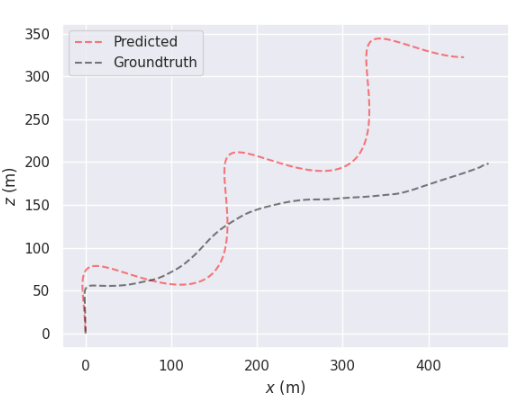
\includegraphics[width=0.8\textwidth]{./images/6_1_trajectory_3_encoder_only}
    \caption{Sequence 3 predicted by encoder-only model}
    \label{fig:trajectory-3-encoder-only}
\end{figure}

After a few trials with encoder-decoder model, which produced some circular trajectories, feeding the \textit{sequence 3} of KITTI (for more details \S~\ref{sec:kitti}) where the first pose of the sequence is considered as origin, we showed that the model (with both 6 and 12 layers of encoder-decoder) is able to learn a single sequence in over-fitting, but fails when trying to over-fit a more complex sequence.
The same model succeeded also in predicting the sequence 7, but failed when we combined the two sequences.
It also fails when we try to over-fit the most complicate sequence, the sequence 0.
\begin{figure}[H]
    \centering
    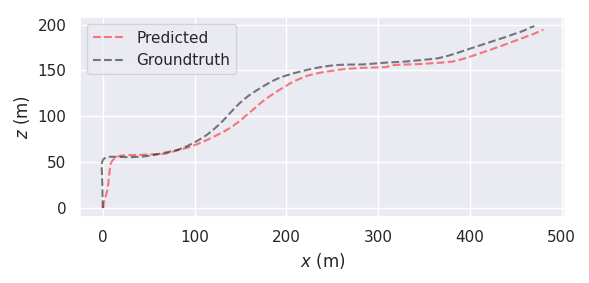
\includegraphics[width=0.8\textwidth]{images/6_1_well_predicted_seq_3}
    \caption{Good prediction sequence 3}\label{fig:well-predicted-seq-3}
\end{figure}
\begin{figure}[H]
    \centering
    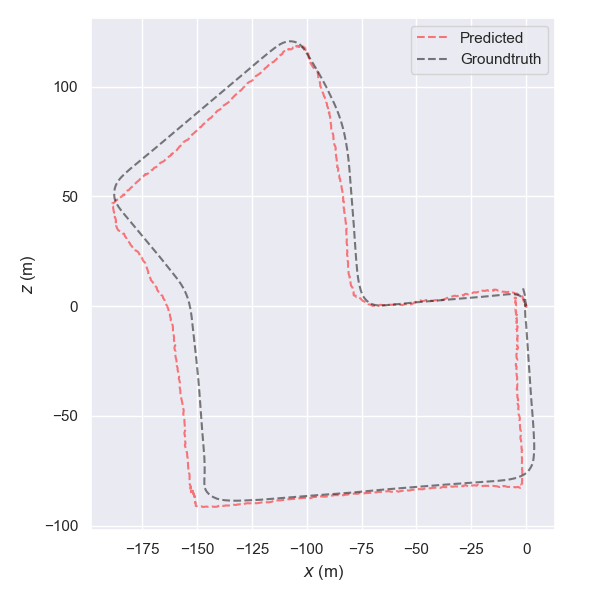
\includegraphics[width=0.8\textwidth]{images/6_1_well_predicted_seq_7}
    \caption{Good prediction sequence 7}\label{fig:well-predicted-seq-7}
\end{figure}
% %**************************************************************

\subsection{Autoregressive models}\label{subsec:autoregressive-model}
We implemented only the encoder-decoder version of the transformer in the autoregressive way, and most of the time the prediction of the network during the training on seq 3 is just a straight line.
So the model is \textbf{not} able to predict the simplest sequence in over-fitting.
The model could not predict any reasonable trajectory, predicting only a linear trajectory as the follow:
\begin{figure}[H]
    \centering
    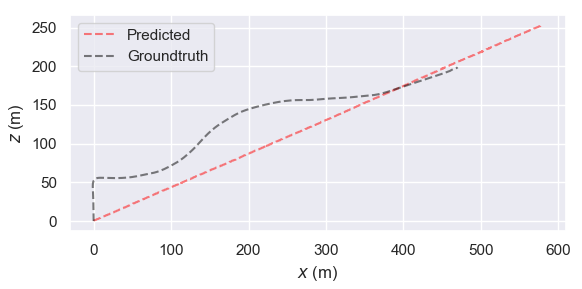
\includegraphics[width=0.8\textwidth]{images/6_1_autoregressive_prediction}
    \caption{Bad prediction sequence 3 of autoregressive model}\label{fig:autoregressive-seq-3}
\end{figure}
Although the model has been trained for more than two hundred epochs, the network cannot understand the goal, and this maybe is due to the loss function.

%**************************************************************

%\section{Knowledge acquired}\label{sec:knowledge-acquired}
By developing this project, I amplified my knowledge with various topics, such as:
\begin{itemize}
    \item Deep Learning,
    \item Computer Vision.
    \item Anaconda.
    \item PyTorch.
    \item Transformers.
    \item Auto-regressive models.
\end{itemize}
Especially, how the transformer works, and how to use it for computer vision tasks.
At the beginning of the project, the word ``transformer'' has had other meanings, but now, I know that it is a neural network architecture that is able to learn the sequence of images and the sequence of poses in a self-supervised way.
It's a general purpose architecture for domain adaptation from one sequence to another.
Another important notion that I learned is the concept of auto-regressive models.

To develop this approach, I had to deepen my knowledge about Visual Odometry, especially, a solid understanding of the task, basis knowledge such as the pose representations and the conversion between them.
I also had to amply my knowledge about the deep-learning framework, PyTorch, specifically, how to build a model, which are the components that are provided by the library, and how to use them.
For example, I had to implement the Transformer, initially I was implementing it from scratch, but then I discovered that there was some classes already implemented in the library, so I used latter ones, because they are more efficient and they are already tested.
I had to use Anaconda to manage the Python environment, because it is a very useful tool, and it is very easy to use.


%**************************************************************

\section{Future developments}\label{sec:future-developments}

During the training process, the loss function often converges to the minimum value at about 200 epoch.
But it does not decrease anymore, and the trajectory does not improve anymore.
So, we should use a different loss function instead of the one used, MSE o WSME, because they are not suitable for this task.
An ideal loss function for this task should describe the error in a way that the network can understand.

Another problem is that we do not have a large amount of data, so we should create synthetic dataset which is more suitable for this task.
For example, we can follow the approach adopted by Richter et al. (\cite{synthetic_dataset}), in this way we can create a dataset with a large number of images and poses.
Then, use it for pre-training, and finally, use the real KITTI dataset for fine-tuning.

We should also try with a different feature extractor, because the ResNets are designed for the classification task, and the embedding produced describes the image as whole, losing local information.
This is because the use of pooling layers, which are used to guarantee the translation invariance of the network when performing the classification or object detection tasks.
Meanwhile, for a task like VO this translation invariance is harmful, because it does not allow the network to learn the local features of the image.
The approach adopted by Dosovitsky et al. (\cite{vit_paper}), which consisted in split the image in smaller patches, then extract the embedding for each patch, and then combine them, could be a good solution.

Another experiment could be to change totally the feeding strategy, using a pair of images stacked together as did in many approaches, for example in ~\cite{deep_vo}.
In the same way, we can try to use the optical flow of the input images to help the network to understand the local motion.

As last attempt, it would be useful to try to use a RNN as prediction head, because it is able to learn the temporal information, and it can predict the next pose given the previous ones, also because, in the literature, good results have been reached using RNNs.

%**************************************************************

\section{Personal Evaluation}\label{sec:personal-evaluation}
By doing this project, I learned a new way-of-working and I improved my knowledge in various topics and fields.
I think this is very educational, and it introduced me into the world of research, letting me know that not every trial is successful, and that it is necessary to be meticulous and to have a lot of patience if you want to achieve good results.
I also learned that it is necessary to have a good knowledge of the topic, and to have a solid background, to do a lot of researches and to read a lot of papers, to understand the problem and to find the best solution.

It has been an interesting experience, and I think that I have learned a lot, improving my abilities to work with neural networks, to fix their problem and to see the results in a critical way.

Finally, I would like to thank my supervisor, Prof.~Luigi Di Stefano and my co-supervisor, Luca De Luigi for being so helpful and patient to help me to complete this project.
Without their help, I would not have been able to complete this project.

%**************************************************************

    %**************************************************************
    % Materiale finale
    %**************************************************************
    \backmatter
    \newpage
    ~\newpage
    \printglossaries
    % !TEX encoding = UTF-8
% !TEX TS-program = pdflatex
% !TEX root = ../tesi.tex

%**************************************************************
% Ringraziamenti
%**************************************************************
\cleardoublepage
\phantomsection
\pdfbookmark{Acknowledgements}{Acknowledgements}


%\bigskip

\begingroup
\let\clearpage\relax
\let\cleardoublepage\relax
\let\cleardoublepage\relax

\chapter*{Acknowledgements}

\noindent First, I would like to express my deepest gratitude to Professor Calegari and Professor Ciatto for all the support they provided me during the internship and thesis redaction processes.\\

\noindent Second, I would like to thank my family, my friends and all people who believed in me during this long study path.\\


\noindent Last but not least, I would like to thank myself to have been able to never give up during these two years. \\

\noindent\textit{\myLocation, \myTime}
\hfill \myName

\endgroup


    % !TEX encoding = UTF-8
% !TEX TS-program = pdflatex
% !TEX root = ../tesi.tex

%**************************************************************
% Bibliografia
%**************************************************************

\cleardoublepage
% \chapter{Bibliopraphy}\label{ch:bibliografia}

\nocite{*}
% Stampa i riferimenti bibliografici
\printbibliography
%\printbibliography[heading=subbibliography,title={Bibliography references},type=book]

% Stampa i siti web consultati
%\printbibliography[heading=subbibliography,title={Website references},type=online]
%\printbibliography[heading=subbibliography,title={Paper references},type=article]


\end{document}
